% ============================================================
% 平均分散から Black-Litterman へ（勉強用）
% コンパイル：tectonic BLM解説.tex   （XeTeX 系）
% 数値・表・図は BLM解説_計算.py が BLM解説_生成/ に作る。先にそれを実行すること:
%   （リポジトリの直下で）.venv/bin/python 資料集/勉強用/BLM解説_計算.py
% ============================================================
\documentclass[xelatex,ja=standard,jafont=hiragino-pron,a4paper,11pt,openany]{bxjsreport}
\setpagelayout*{left=22mm,right=22mm,top=22mm,bottom=25mm,footskip=11mm}

\usepackage{amsmath,amssymb,mathtools,bm}
\usepackage{booktabs,array,multirow}
\usepackage{graphicx}
\usepackage{adjustbox}
\usepackage{xcolor}
\usepackage{tikz}
\usetikzlibrary{arrows.meta,positioning,calc}
\usepackage{listings}
\usepackage{enumitem}
\usepackage{caption}
\usepackage[most]{tcolorbox}
\usepackage[hidelinks,bookmarksnumbered]{hyperref}

\graphicspath{{BLM解説_生成/}}

% ---- 色（総合報告書と同じ）
\definecolor{c1}{HTML}{2A78D6}
\definecolor{c2}{HTML}{EB6834}
\definecolor{c3}{HTML}{1BAF7A}
\definecolor{c4}{HTML}{EDA100}
\definecolor{c7}{HTML}{6250D6}
\definecolor{ink2}{HTML}{52514E}
\definecolor{soft1}{HTML}{E4EEF9}
\definecolor{soft2}{HTML}{FBEEDF}
\definecolor{soft3}{HTML}{E3F3E9}
\definecolor{soft4}{HTML}{EEE8FA}

% ---- 計算で作った数値（\V{名前}）
% BLM解説_計算.py が作ったファイル（手で直さない）
\expandafter\def\csname v@toy.muA\endcsname{6}
\expandafter\def\csname v@toy.sA\endcsname{20}
\expandafter\def\csname v@toy.muB\endcsname{2}
\expandafter\def\csname v@toy.sB\endcsname{10}
\expandafter\def\csname v@toy.rho\endcsname{0.3}
\expandafter\def\csname v@toy.covAB\endcsname{0.0060}
\expandafter\def\csname v@toy.varA\endcsname{0.04}
\expandafter\def\csname v@toy.varB\endcsname{0.01}
\expandafter\def\csname v@toy.mp\endcsname{4.0}
\expandafter\def\csname v@toy.vp\endcsname{0.0155}
\expandafter\def\csname v@toy.sp\endcsname{12.45}
\expandafter\def\csname v@toy.vpA\endcsname{0.0100}
\expandafter\def\csname v@toy.vpB\endcsname{0.0025}
\expandafter\def\csname v@toy.vpAB\endcsname{0.0030}
\expandafter\def\csname v@toy.wone\endcsname{0.60}
\expandafter\def\csname v@toy.det\endcsname{0.000364}
\expandafter\def\csname v@toy.Si00\endcsname{27.47}
\expandafter\def\csname v@toy.Si01\endcsname{\ensuremath{-}16.48}
\expandafter\def\csname v@toy.Si11\endcsname{109.89}
\expandafter\def\csname v@toy.Simu0\endcsname{1.3187}
\expandafter\def\csname v@toy.Simu1\endcsname{1.2088}
\expandafter\def\csname v@toy.wfreeA\endcsname{0.5275}
\expandafter\def\csname v@toy.wfreeB\endcsname{0.4835}
\expandafter\def\csname v@toy.wfreesum\endcsname{1.0110}
\expandafter\def\csname v@toy.wfreeApct\endcsname{52.7}
\expandafter\def\csname v@toy.wfreeBpct\endcsname{48.4}
\expandafter\def\csname v@toy.wfreecash\endcsname{\ensuremath{-}1.1}
\expandafter\def\csname v@toy.oneSimu\endcsname{2.5275}
\expandafter\def\csname v@toy.oneSione\endcsname{104.40}
\expandafter\def\csname v@toy.gamma\endcsname{0.03}
\expandafter\def\csname v@toy.gammaraw\endcsname{0.00026}
\expandafter\def\csname v@toy.wbudA\endcsname{52.6}
\expandafter\def\csname v@toy.wbudB\endcsname{47.4}
\expandafter\def\csname v@toy.wbudA7\endcsname{63.2}
\expandafter\def\csname v@toy.wbudB7\endcsname{36.8}
\expandafter\def\csname v@g7.SwGER\endcsname{0.036109}
\expandafter\def\csname v@g7.PiGER\endcsname{9.03}
\expandafter\def\csname v@g7.PiGERraw\endcsname{0.09027}
\expandafter\def\csname v@g7.SGERGER\endcsname{0.07344}
\expandafter\def\csname v@g7.varm\endcsname{0.02854}
\expandafter\def\csname v@g7.sigm\endcsname{16.89}
\expandafter\def\csname v@g7.Pim\endcsname{7.13}
\expandafter\def\csname v@g7.sharpe\endcsname{0.422}
\expandafter\def\csname v@g7.deltacheck\endcsname{2.500}
\expandafter\def\csname v@sens.gerup\endcsname{29.1}
\expandafter\def\csname v@sens.fraup\endcsname{\ensuremath{-}10.8}
\expandafter\def\csname v@sens.ukup\endcsname{6.2}
\expandafter\def\csname v@sens.gerfr\endcsname{45.1}
\expandafter\def\csname v@sens.frafr\endcsname{\ensuremath{-}41.1}
\expandafter\def\csname v@sens.eqmin\endcsname{\ensuremath{-}22.3}
\expandafter\def\csname v@sens.eqmax\endcsname{47.5}
\expandafter\def\csname v@sens.eqminname\endcsname{ドイツ}
\expandafter\def\csname v@sens.eqmaxname\endcsname{オーストラリア}
\expandafter\def\csname v@sc.pi\endcsname{5}
\expandafter\def\csname v@sc.sig\endcsname{20}
\expandafter\def\csname v@sc.tau\endcsname{0.05}
\expandafter\def\csname v@sc.q\endcsname{10}
\expandafter\def\csname v@sc.ts\endcsname{0.002}
\expandafter\def\csname v@sc.tssd\endcsname{4.47}
\expandafter\def\csname v@sc.post\endcsname{7.50}
\expandafter\def\csname v@sc.postsd\endcsname{3.16}
\expandafter\def\csname v@ex1.pFRA\endcsname{\ensuremath{-}0.2955}
\expandafter\def\csname v@ex1.pUK\endcsname{\ensuremath{-}0.7045}
\expandafter\def\csname v@ex1.pPi\endcsname{1.79}
\expandafter\def\csname v@ex1.gap\endcsname{3.21}
\expandafter\def\csname v@ex1.pSp\endcsname{0.02130}
\expandafter\def\csname v@ex1.ptSp\endcsname{0.001065}
\expandafter\def\csname v@ex1.omega\endcsname{0.001065}
\expandafter\def\csname v@ex1.viewsd\endcsname{3.26}
\expandafter\def\csname v@ex1.pmu\endcsname{3.39}
\expandafter\def\csname v@ex1.lam\endcsname{0.317}
\expandafter\def\csname v@ex1.lamscaled\endcsname{0.302}
\expandafter\def\csname v@ex1.Mratio\endcsname{0.879}
\expandafter\def\csname v@ex1.qzero\endcsname{1.70}
\expandafter\def\csname v@ex1.A\endcsname{0.04158}
\expandafter\def\csname v@ex1.omtau\endcsname{0.02130}
\expandafter\def\csname v@ex1.pSptau\endcsname{0.02028}
\expandafter\def\csname v@ex1.d\endcsname{3.30}
\expandafter\def\csname v@ex1.dA\endcsname{0.10396}
\expandafter\def\csname v@ex1.lamAtpPi\endcsname{0.0082}
\expandafter\def\csname v@ex2.p2Pi\endcsname{\ensuremath{-}0.64}
\expandafter\def\csname v@ex2.gap2\endcsname{3.64}
\expandafter\def\csname v@ex2.lamA\endcsname{0.298}
\expandafter\def\csname v@ex2.lamB\endcsname{0.418}
\expandafter\def\csname v@ex2.p1mu\endcsname{3.50}
\expandafter\def\csname v@ex2.p2mu\endcsname{1.25}
\expandafter\def\csname v@ex2.omegaA\endcsname{0.001065}
\expandafter\def\csname v@ex2.omegaB\endcsname{0.000852}
\expandafter\def\csname v@ex2.viewcorr\endcsname{0.105}
\expandafter\def\csname v@ex2.wsum\endcsname{95.2}
\expandafter\def\csname v@ex2.w1sum\endcsname{95.2}
\expandafter\def\csname v@ex2.CAN\endcsname{41.9}
\expandafter\def\csname v@ex2.USA\endcsname{18.8}
\expandafter\def\csname v@ex3.lamA\endcsname{0.292}
\expandafter\def\csname v@ex3.lamB\endcsname{0.538}
\expandafter\def\csname v@ex4.lamA\endcsname{0.193}
\expandafter\def\csname v@ex4.lamB\endcsname{0.544}
\expandafter\def\csname v@ex4.p1mu\endcsname{3.04}
\expandafter\def\csname v@ex3.p1mu\endcsname{3.53}
\expandafter\def\csname v@ex5.qstar\endcsname{\ensuremath{-}0.46}
\expandafter\def\csname v@ex5.lamA\endcsname{0.317}
\expandafter\def\csname v@ex5.lamB\endcsname{0.000}
\expandafter\def\csname v@ex5.p2Pi\endcsname{\ensuremath{-}0.64}
\expandafter\def\csname v@ex5.p2Pitau\endcsname{\ensuremath{-}0.61}
\expandafter\def\csname v@ex5.p2mu1\endcsname{\ensuremath{-}0.49}
\expandafter\def\csname v@ex5.p2mu1tau\endcsname{\ensuremath{-}0.47}
\expandafter\def\csname v@ex5.slope\endcsname{0.121}
\expandafter\def\csname v@lo.CAN\endcsname{41.7}
\expandafter\def\csname v@lo.GER\endcsname{27.5}
\expandafter\def\csname v@lo.USA\endcsname{17.4}
\expandafter\def\csname v@lo.diffSSp\endcsname{2.26}
\expandafter\def\csname v@cfg.tau\endcsname{0.025}
\expandafter\def\csname v@cfg.delta\endcsname{2.5}
\expandafter\def\csname v@cfg.window\endcsname{252}
\expandafter\def\csname v@cfg.minhist\endcsname{0.5}
\expandafter\def\csname v@cfg.origrf\endcsname{0.02}
\expandafter\def\csname v@cfg.origrw\endcsname{0.1}
\expandafter\def\csname v@pj.date\endcsname{2025-01-31}
\expandafter\def\csname v@pj.rf\endcsname{0.0166}
\expandafter\def\csname v@pj.rfyear\endcsname{4.19}
\expandafter\def\csname v@pj.N\endcsname{487}
\expandafter\def\csname v@pj.days\endcsname{252}
\expandafter\def\csname v@pj.mdays\endcsname{20}
\expandafter\def\csname v@pj.alpha5\endcsname{0.048}
\expandafter\def\csname v@pj.target5\endcsname{3.921}
\expandafter\def\csname v@pj.var5\endcsname{2.411}
\expandafter\def\csname v@pj.Pim5\endcsname{0.0603}
\expandafter\def\csname v@pj.Pim5year\endcsname{15.2}
\expandafter\def\csname v@pj.sigm5year\endcsname{24.6}
\expandafter\def\csname v@pj.PiAAPL\endcsname{0.0345}
\expandafter\def\csname v@pj.SwAAPL\endcsname{1.379}
\expandafter\def\csname v@pj.PiJNJ\endcsname{\ensuremath{-}0.0120}
\expandafter\def\csname v@pj.betaJNJ\endcsname{\ensuremath{-}0.20}
\expandafter\def\csname v@pj.PiNVDA\endcsname{0.1227}
\expandafter\def\csname v@pj.aaplmean\endcsname{\ensuremath{-}0.291}
\expandafter\def\csname v@pj.aaplsd\endcsname{0.130}
\expandafter\def\csname v@pj.aaplvar\endcsname{1.689}
\expandafter\def\csname v@pj.aaplmon\endcsname{\ensuremath{-}0.278}
\expandafter\def\csname v@pj.kmin\endcsname{0.59}
\expandafter\def\csname v@pj.kmax\endcsname{0.94}
\expandafter\def\csname v@pj.formdiff\endcsname{\ensuremath{1.4\times 10^{-18}}}
\expandafter\def\csname v@pj.QAAPL\endcsname{\ensuremath{-}0.3079}
\expandafter\def\csname v@pj.muAAPL\endcsname{\ensuremath{-}0.2224}
\expandafter\def\csname v@pj.QJPM\endcsname{0.5294}
\expandafter\def\csname v@pj.muJPM\endcsname{0.4496}
\expandafter\def\csname v@pj.moveXOM\endcsname{0.113}
\expandafter\def\csname v@pj.kXOM\endcsname{0.587}
\expandafter\def\csname v@pj.QXOM\endcsname{\ensuremath{-}0.1077}
\expandafter\def\csname v@pj.muXOM\endcsname{\ensuremath{-}0.0126}
\expandafter\def\csname v@pj.PiXOM\endcsname{\ensuremath{-}0.0004}
\expandafter\def\csname v@pj.tsAA\endcsname{5.590}
\expandafter\def\csname v@pj.omAA\endcsname{1.689}
\expandafter\def\csname v@pj.kAA\endcsname{0.768}
\expandafter\def\csname v@pj.diagAAPL\endcsname{\ensuremath{-}0.2284}
\expandafter\def\csname v@pj.gapAAPL\endcsname{\ensuremath{-}0.3423}
\expandafter\def\csname v@pj.eqcheck\endcsname{\ensuremath{2.6\times 10^{-8}}}
\expandafter\def\csname v@pj.wfreesum\endcsname{739}
\expandafter\def\csname v@pj.penJPM\endcsname{0.0571}
\expandafter\def\csname v@pj.corrXOMJPM\endcsname{0.31}
\expandafter\def\csname v@pj.wblNVDA\endcsname{0.0}
\expandafter\def\csname v@pj.wblJPM\endcsname{100.0}
\expandafter\def\csname v@pj.wblJNJ\endcsname{0.0}
\expandafter\def\csname v@pj.wblAAPL\endcsname{0.0}
\expandafter\def\csname v@pj.wblXOM\endcsname{0.0}
\expandafter\def\csname v@pj.lamAAPL\endcsname{\ensuremath{-}5.15}
\expandafter\def\csname v@pj.lamJPM\endcsname{7.70}
\expandafter\def\csname v@or.mktmean\endcsname{\ensuremath{-}0.210}
\expandafter\def\csname v@or.prem\endcsname{\ensuremath{-}2.210}
\expandafter\def\csname v@or.days\endcsname{20}
\expandafter\def\csname v@or.nit\endcsname{1}
\expandafter\def\csname v@or.f0\endcsname{\ensuremath{2.7\times 10^{-5}}}
\expandafter\def\csname v@or.fexact\endcsname{\ensuremath{\ensuremath{-}2.2\times 10^{-4}}}
\expandafter\def\csname v@or.wJPMexact\endcsname{100.0}
\expandafter\def\csname v@or.PiAAPL\endcsname{\ensuremath{-}0.829}
\expandafter\def\csname v@z.muA\endcsname{0.1877}
\expandafter\def\csname v@z.muB\endcsname{0.2000}
\expandafter\def\csname v@z.muAo\endcsname{0.1845}
\expandafter\def\csname v@z.muBo\endcsname{0.0686}
\expandafter\def\csname v@z.minvar\endcsname{\ensuremath{3.6\times 10^{-8}}}
\expandafter\def\csname v@all.alpha\endcsname{0.118}
\expandafter\def\csname v@all.storeddiff\endcsname{0.000}
\expandafter\def\csname v@all.ratiomed\endcsname{0.215}
\expandafter\def\csname v@all.ratioq1\endcsname{0.135}
\expandafter\def\csname v@all.ratioq3\endcsname{0.324}
\expandafter\def\csname v@all.kmed\endcsname{0.823}
\expandafter\def\csname v@all.kq1\endcsname{0.755}
\expandafter\def\csname v@all.kq3\endcsname{0.881}
\expandafter\def\csname v@all.movemed\endcsname{0.939}
\expandafter\def\csname v@all.corrQ\endcsname{0.956}
\expandafter\def\csname v@all.corrPi\endcsname{0.347}
\expandafter\def\csname v@all.Pimed\endcsname{0.0102}
\expandafter\def\csname v@all.Qmed\endcsname{0.229}
\expandafter\def\csname v@all.Qsd\endcsname{0.291}
\expandafter\def\csname v@all.Pisd\endcsname{0.0081}
\expandafter\def\csname v@all.shareBig\endcsname{90}
\expandafter\def\csname v@all.topQmonth\endcsname{41}
\expandafter\def\csname v@all.topQ\endcsname{1.65}
\expandafter\def\csname v@all.topname\endcsname{VST}
\expandafter\def\csname v@all.sdmed\endcsname{1.63}
\expandafter\def\csname v@all.semonth\endcsname{0.356}
\expandafter\def\csname v@all.effmkt\endcsname{53.2}
\expandafter\def\csname v@all.effbl\endcsname{1.63}
\expandafter\def\csname v@all.nheld\endcsname{2}
\expandafter\def\csname v@dates.n\endcsname{30}
\expandafter\def\csname v@dates.kmin\endcsname{0.75}
\expandafter\def\csname v@dates.kmax\endcsname{0.91}
\expandafter\def\csname v@dates.rmin\endcsname{0.10}
\expandafter\def\csname v@dates.rmax\endcsname{0.33}

\newcommand{\V}[1]{\ifcsname v@#1\endcsname\csname v@#1\endcsname\else\textbf{??#1??}\fi}
\newcommand{\tabin}[1]{\adjustbox{max width=\linewidth}{\input{BLM解説_生成/tab_#1.tex}}}

% ---- よく使う表記
\newcommand{\code}[1]{\texttt{#1}}
\newcommand{\SP}{S\&P500}
\newcommand{\T}{^{\top}}
\newcommand{\weq}{w_{\mathrm{eq}}}
\newcommand{\mub}{\bar{\mu}}
\newcommand{\Sp}{\Sigma_{p}}
\newcommand{\one}{\mathbf{1}}
\DeclareMathOperator{\diag}{diag}
\newcommand{\figref}[1]{図~\ref{#1}}
\newcommand{\tabref}[1]{表~\ref{#1}}
\newcommand{\chapref}[1]{第~\ref{#1}~章}
\newcommand{\secref}[1]{\ref{#1}~節}

\setlist[itemize]{leftmargin=1.6em,itemsep=0.2em,topsep=0.4em}
\setlist[enumerate]{leftmargin=1.8em,itemsep=0.2em,topsep=0.4em}
\captionsetup{font=small,labelfont=bf,skip=6pt}
\renewcommand{\arraystretch}{1.2}

% ---- 図表の置き方（余白を減らす）
\renewcommand{\topfraction}{0.85}
\renewcommand{\bottomfraction}{0.7}
\renewcommand{\textfraction}{0.1}
\renewcommand{\floatpagefraction}{0.75}
\setcounter{totalnumber}{4}

% ---- 章の見出しを小さくする
\makeatletter
\def\@makechapterhead#1{\vspace*{0.3\Cvs}{\parindent\z@\raggedright\normalfont
  \ifnum\c@secnumdepth>\m@ne\if@mainmatter{\Large\headfont\@chapapp\thechapter\@chappos}\par\nobreak\vskip0.4\Cvs\fi\fi
  \interlinepenalty\@M\LARGE\headfont #1\par\nobreak\vskip 1.5\Cvs}}
\def\@makeschapterhead#1{\vspace*{0.3\Cvs}{\parindent\z@\raggedright\normalfont
  \interlinepenalty\@M\LARGE\headfont #1\par\nobreak\vskip 1.5\Cvs}}
\makeatother

% ---- コード
\renewcommand{\lstlistingname}{リスト}
\lstset{basicstyle=\ttfamily\footnotesize,breaklines=true,columns=fullflexible,keepspaces=true,
  showstringspaces=false,frame=single,framerule=0.3pt,rulecolor=\color{black!25},backgroundcolor=\color{black!3},
  xleftmargin=3pt,xrightmargin=3pt,aboveskip=8pt,belowskip=8pt,captionpos=t,
  commentstyle=\color{ink2},keywordstyle=\color{c1},stringstyle=\color{c2!80!black}}

% ---- 囲み
\newtcolorbox{keybox}[1][要点]{enhanced,breakable,colback=soft1,colframe=c1,boxrule=0.5pt,arc=2pt,
  left=8pt,right=8pt,top=6pt,bottom=6pt,title={#1},fonttitle=\sffamily\bfseries\small,coltitle=white}
\newtcolorbox{notebox}[1][注意]{enhanced,breakable,colback=soft2,colframe=c2,boxrule=0.5pt,arc=2pt,
  left=8pt,right=8pt,top=6pt,bottom=6pt,title={#1},fonttitle=\sffamily\bfseries\small,coltitle=white}
\newtcolorbox{exbox}[1][計算例]{enhanced,breakable,colback=soft3,colframe=c3,boxrule=0.5pt,arc=2pt,
  left=8pt,right=8pt,top=6pt,bottom=6pt,title={#1},fonttitle=\sffamily\bfseries\small,coltitle=white}
\newtcolorbox{thmbox}[1][結果]{enhanced,breakable,colback=soft4,colframe=c7,boxrule=0.5pt,arc=2pt,
  left=8pt,right=8pt,top=6pt,bottom=6pt,title={#1},fonttitle=\sffamily\bfseries\small,coltitle=white}

% ---- 図の部品
\tikzset{
  box/.style={draw=#1,fill=#1!8,rounded corners=2pt,align=center,font=\footnotesize,inner sep=4pt,
              minimum height=11mm,text width=27mm},
  arr/.style={-{Stealth[length=2mm]},color=ink2,line width=0.6pt},
  lab/.style={font=\scriptsize,color=ink2},
}

\title{平均分散から Black-Litterman へ\\[6pt]
  \large He と Litterman（1999）に沿った解説と、本プロジェクト（LLM-BLM）の計算}
\author{勉強用資料}
\date{2026 年 10 月}

\begin{document}
\maketitle
\setcounter{tocdepth}{1}
{\small\tableofcontents}

% ============================================================
\chapter*{この資料について}
\addcontentsline{toc}{chapter}{この資料について}

この資料は、本プロジェクト（LLM-BLM）の比率の計算（\code{blm/}）が何をしているかを、平均分散最適化から順に、式と具体的な数字で追うためのものである。

骨組みには、He と Litterman の論文 \textit{The Intuition Behind Black-Litterman Model Portfolios}（1999 年、Goldman Sachs Investment Management Research）を使う。Black-Litterman モデル（以下 BL）の原論文（Black and Litterman 1992）は、結果の数字を中心に書かれていて、式の導き方や、出てくる比率がなぜその形になるのかの説明は少ない。He と Litterman は、BL で得られる最適ポートフォリオが
\begin{center}
「市場ポートフォリオ」＋「ビューを表すポートフォリオの重み付きの和」
\end{center}
という形で書けることを示し、G7 の株式市場の例で、ビューの強さや自信の度合いが比率にどう効くかを 1 つずつ確かめた。この資料も同じ順に進み、同じデータで計算をやり直す。

\section*{構成}

\begin{center}
\small
\begin{tabular}{p{2.0cm}p{11.2cm}}
\toprule
章 & 内容 \\
\midrule
第 1 章 & 平均分散最適化。2 資産の例で、比率の公式と、その弱点を見る \\
第 2 章 & 市場の均衡リターン（逆最適化）。G7 の例で計算する \\
第 3 章 & ビュー（投資家の見方）を $P$、$Q$、$\Omega$ で表す \\
第 4 章 & 均衡とビューをベイズの考え方で混ぜる。BL の公式を導き、G7 の例を手で計算する \\
第 5 章 & He と Litterman の主結果。最適ポートフォリオの形と、その 4 つの性質 \\
第 6 章 & 実際に使うときの論点（制約、$\tau$ の意味、単位、共分散の推定） \\
第 7 章 & 本プロジェクトの計算。5 銘柄の実データで、コードと同じ計算を 1 段ずつ追う \\
第 8 章 & まとめ \\
付録 & 行列の公式、本プロジェクトのコード、参考文献 \\
\bottomrule
\end{tabular}
\end{center}

前提として、行列の積と逆行列、正規分布、偏微分を使う。使う公式は付録 A にまとめた。

\section*{数字の出どころ}

本文と表の数字は、すべて同じフォルダの \code{BLM解説\_計算.py} で計算し、自動で差し込んでいる（手で写した数字はない）。

\begin{itemize}
\item \textbf{G7 の例}：入力（相関、標準偏差、時価総額の比率）は He と Litterman の表 1 の値（もとは Black and Litterman 1992 の値）を使った。この入力から均衡リターンを計算し直すと、論文の表 1 の値と小数 1 桁まで一致する（\tabref{tab:g7inputs}）。それ以降の例の数字は、この資料で計算し直したものである。論文の表とは、丸め方の違いで最後の桁がずれることがある。
\item \textbf{本プロジェクトの例}：\code{data/blm.sqlite} の株価と、LLM の回答（LLM の実行番号 1、gpt-4o-mini、1 銘柄につき 30 回答）を使った。判断日は \V{pj.date} である。
\end{itemize}

\section*{記号}

\begin{center}
\small
\begin{tabular}{p{2.6cm}p{1.8cm}p{8.6cm}}
\toprule
記号 & 大きさ & 意味 \\
\midrule
$N$ & & 資産（銘柄）の数 \\
$K$ & & ビューの数 \\
$r$ & $N$ & 資産のリターン（確率変数） \\
$\mu$ & $N$ & 期待リターン。断りがなければ、無リスク金利を引いた超過リターン \\
$\Sigma$ & $N \times N$ & リターンの共分散行列 \\
$w$ & $N$ & 投資比率 \\
$\delta$ & スカラー & リスク回避度 \\
$\weq$ & $N$ & 市場の比率（時価総額の比率） \\
$\Pi$ & $N$ & 均衡リターン $\Pi = \delta\Sigma\weq$ \\
$\tau$ & スカラー & 均衡リターンの不確かさの大きさ \\
$P$ & $K \times N$ & ビューの行列。$k$ 行目 $p_k$ がビュー $k$ のポートフォリオ \\
$Q$ & $K$ & ビューの値 \\
$\Omega$ & $K \times K$ & ビューの不確かさ（共分散）。ふつうは対角行列 \\
$\mub$ & $N$ & BL の事後の期待リターン \\
$M$ & $N \times N$ & 事後の期待リターンの不確かさ（共分散） \\
$\Sp = \Sigma + M$ & $N \times N$ & 予測に使う共分散 \\
$\Lambda = (\lambda_k)$ & $K$ & ビューのポートフォリオに付く重み \\
$\one$ & $N$ & 成分がすべて 1 のベクトル \\
$x\T$ & & 転置 \\
\bottomrule
\end{tabular}
\end{center}

ベクトルはすべて縦ベクトルとする。たとえば $w\T\mu = \sum_i w_i \mu_i$ である。

% ============================================================
\chapter{平均分散最適化}\label{ch:mv}

BL は、平均分散最適化の「入力の作り方」を変える方法である。そこでまず、平均分散最適化そのものと、その弱点を確認する。

\section{ポートフォリオのリターンとリスク}

$N$ 個の資産のリターンを並べたベクトルを $r$ とし、その期待値を $\mu = E[r]$、共分散行列を $\Sigma = \mathrm{Cov}(r)$ とする。$\Sigma$ の $(i,j)$ 成分は資産 $i$ と $j$ のリターンの共分散 $\sigma_{ij} = \rho_{ij}\sigma_i\sigma_j$ で、対角成分は各資産の分散 $\sigma_i^2$ である。

資産 $i$ に比率 $w_i$ を投資したポートフォリオのリターンは $r_p = \sum_i w_i r_i = w\T r$ で、その期待値と分散は
\begin{align}
E[r_p] &= \sum_i w_i \mu_i = w\T\mu, \label{eq:pmean}\\
\mathrm{Var}(r_p) &= \sum_i\sum_j w_i w_j \sigma_{ij} = w\T\Sigma w \label{eq:pvar}
\end{align}
となる。分散の式は、$\mathrm{Var}(\sum_i w_i r_i) = \sum_i \sum_j w_i w_j \mathrm{Cov}(r_i, r_j)$ を行列で書いたものである。

\begin{exbox}[計算例 1.1：2 資産のポートフォリオ]
資産 A は期待リターン \V{toy.muA}\%、標準偏差 \V{toy.sA}\%、資産 B は期待リターン \V{toy.muB}\%、標準偏差 \V{toy.sB}\%、相関は $\rho = \V{toy.rho}$ とする（年率）。共分散は $\sigma_{AB} = 0.3 \times 0.20 \times 0.10 = \V{toy.covAB}$ なので
\[
\mu = \begin{pmatrix} 0.06 \\ 0.02 \end{pmatrix},\qquad
\Sigma = \begin{pmatrix} \V{toy.varA} & \V{toy.covAB} \\ \V{toy.covAB} & \V{toy.varB} \end{pmatrix}.
\]
半分ずつ持つ $w = (0.5,\,0.5)\T$ では、期待リターンは $0.5 \times 6\% + 0.5 \times 2\% = \V{toy.mp}\%$、分散は
\[
w\T\Sigma w = \underbrace{0.5^2 \times 0.04}_{\V{toy.vpA}} + \underbrace{0.5^2 \times 0.01}_{\V{toy.vpB}} + \underbrace{2 \times 0.5 \times 0.5 \times 0.006}_{\V{toy.vpAB}} = \V{toy.vp}
\]
で、標準偏差は $\sqrt{\V{toy.vp}} = \V{toy.sp}\%$ である。
\end{exbox}

標準偏差の単純な平均は $(20\% + 10\%)/2 = 15\%$ だが、ポートフォリオの標準偏差はそれより小さい。相関が 1 より小さいと、一方が下がるときにもう一方が下がらないことがあり、ぶれが打ち消し合うからである。相関を変えたときの値を\tabref{tab:toyrho}に示す。期待リターンは相関によらず同じで、リスクだけが変わる。これが分散投資の効果である。

\begin{table}[htbp]
\centering
\caption{2 資産を半分ずつ持つポートフォリオの、相関とリスク。}
\label{tab:toyrho}
\small\tabin{toy_rho}
\end{table}

この資料では、断りがなければ $\mu$ は無リスク金利を上回る分（超過リターン）を表す。無リスク資産（短期国債など）にお金を置けば、確実に無リスク金利が得られる。比率の合計 $\one\T w$ が 1 より小さいときは残りを無リスク資産に置き、1 より大きいときはその分を無リスク金利で借りていると考える。

\section{リターンとリスクの釣り合い：効用の最大化}

期待リターンは高いほどよく、分散は小さいほどよい。この 2 つを 1 つの数にまとめるため、次の量（効用）を最大にする比率を求める。
\begin{equation}
U(w) = w\T\mu - \frac{\delta}{2}\, w\T\Sigma w
\label{eq:utility}
\end{equation}
$\delta > 0$ はリスク回避度で、分散 1 単位をリターンに換算するといくらの損になるかを決める。$\delta$ が大きいほど、リスクを嫌う投資家である。

\subsection{1 資産の場合}

資産が 1 つで、残りを無リスク資産に置く場合、$U(w) = w\mu - \frac{\delta}{2} w^2\sigma^2$ である。$w$ で微分して 0 とおくと
\begin{equation}
\frac{dU}{dw} = \mu - \delta w \sigma^2 = 0
\quad\Longrightarrow\quad
w^* = \frac{\mu}{\delta\sigma^2}
\label{eq:one}
\end{equation}
となる。期待リターンが高いほど多く持ち、分散が大きいほど、またリスクを嫌うほど少なく持つ。資産 A だけなら、$\delta = 2.5$ として $w^* = 0.06 / (2.5 \times 0.04) = \V{toy.wone}$、つまり 60\% を A に、40\% を無リスク資産に置くのが最適である。

\subsection{$N$ 資産の場合}

ベクトルで微分すると、$\partial(w\T\mu)/\partial w = \mu$、$\partial(w\T\Sigma w)/\partial w = 2\Sigma w$ なので（付録 A）、
\begin{equation}
\frac{\partial U}{\partial w} = \mu - \delta\Sigma w = 0
\quad\Longrightarrow\quad
w^* = (\delta\Sigma)^{-1}\mu
\label{eq:mvfree}
\end{equation}
となる。式~\eqref{eq:one} の $\mu/(\delta\sigma^2)$ を、そのまま行列にした形である。$\Sigma$ は正定値なので、$U$ は上に凸で、この点が最大になる。

\begin{exbox}[計算例 1.2：2 資産の最適比率（制約なし）]
計算例 1.1 の 2 資産で、$\delta = 2.5$ とする。$2 \times 2$ 行列の逆行列は
\[
\Sigma^{-1} = \frac{1}{\sigma_A^2\sigma_B^2 - \sigma_{AB}^2}
\begin{pmatrix} \sigma_B^2 & -\sigma_{AB} \\ -\sigma_{AB} & \sigma_A^2 \end{pmatrix}
\]
で、行列式は $0.04 \times 0.01 - 0.006^2 = \V{toy.det}$ だから
\[
\Sigma^{-1} = \begin{pmatrix} \V{toy.Si00} & \V{toy.Si01} \\ \V{toy.Si01} & \V{toy.Si11} \end{pmatrix},
\]
\[
\Sigma^{-1}\mu = \begin{pmatrix} \V{toy.Si00} \times 0.06 + (\V{toy.Si01}) \times 0.02 \\ (\V{toy.Si01}) \times 0.06 + \V{toy.Si11} \times 0.02 \end{pmatrix}
= \begin{pmatrix} \V{toy.Simu0} \\ \V{toy.Simu1} \end{pmatrix}.
\]
これを $\delta = 2.5$ で割ると $w^* = (\V{toy.wfreeA},\ \V{toy.wfreeB})\T$ になる。A に \V{toy.wfreeApct}\%、B に \V{toy.wfreeBpct}\% で、合計は \V{toy.wfreesum} なので、足りない 1.1\% を無リスク金利で借りることになる。
\end{exbox}

\section{全額を投資する場合}

無リスク資産を使わず、比率の合計を 1 にする（全額をこれらの資産に投資する）場合は、条件 $\one\T w = 1$ を付けて最大化する。ラグランジュ乗数 $\gamma$ を使って
\[
L(w, \gamma) = w\T\mu - \frac{\delta}{2} w\T\Sigma w - \gamma(\one\T w - 1)
\]
を $w$ で微分して 0 とおくと $\mu - \delta\Sigma w - \gamma\one = 0$、つまり
\begin{equation}
w^* = \frac{1}{\delta}\Sigma^{-1}(\mu - \gamma\one)
\label{eq:mvbudget}
\end{equation}
である。$\gamma$ は、条件 $\one\T w^* = 1$ から
\begin{equation}
\gamma = \frac{\one\T\Sigma^{-1}\mu - \delta}{\one\T\Sigma^{-1}\one}
\label{eq:gamma}
\end{equation}
と決まる。式~\eqref{eq:mvbudget} は、式~\eqref{eq:mvfree} の $\mu$ を、全資産から同じ $\gamma$ を引いた $\mu - \gamma\one$ に置き換えた形である。$\gamma$ は「全額を投資する」という条件のために、すべての資産に一律にかかる基準のリターンだと読める。

\begin{exbox}[計算例 1.3：2 資産の最適比率（全額投資）]
計算例 1.2 の $\Sigma^{-1}$ から、$\one\T\Sigma^{-1}\mu = \V{toy.Simu0} + \V{toy.Simu1} = \V{toy.oneSimu}$、$\one\T\Sigma^{-1}\one = \V{toy.Si00} + 2 \times (\V{toy.Si01}) + \V{toy.Si11} = \V{toy.oneSione}$ なので
\[
\gamma = \frac{\V{toy.oneSimu} - 2.5}{\V{toy.oneSione}} = \V{toy.gammaraw} \;(\approx \V{toy.gamma}\%).
\]
式~\eqref{eq:mvbudget} に入れると、A が \V{toy.wbudA}\%、B が \V{toy.wbudB}\% になる。制約なしの解がもともと合計 1 に近かったので、ほとんど変わらない。

ここで、A の期待リターンを 6\% から 7\% に 1\% だけ上げてみる。同じ計算をやり直すと、A が \V{toy.wbudA7}\%、B が \V{toy.wbudB7}\% になる。期待リターンの 1\% の違いで、比率が 10\% 以上動く。
\end{exbox}

\section{平均分散最適化の弱点}\label{sec:mvweak}

式~\eqref{eq:mvfree} は単純で、理論としては申し分ない。しかし実際に使うと、次の問題が起きることがよく知られている。

\subsection{期待リターンは推定できない}

共分散は、日次のデータを使えば比較的精度よく推定できる。一方、期待リターンの推定は非常に難しい。年率の標準偏差 $\sigma$ の資産の平均リターンを $T$ 年分のデータで推定すると、その標準誤差は $\sigma/\sqrt{T}$ である（日次で測っても、期間の長さ $T$ 年が同じなら精度はほぼ変わらない）。

\begin{table}[htbp]
\centering
\caption{期待リターンの推定の精度（年率の標準偏差 20\% の資産）。}
\label{tab:se}
\small\tabin{se}
\end{table}

\tabref{tab:se} のとおり、10 年分のデータがあっても、95\% の範囲は $\pm 12\%$ 以上ある。期待リターン 6\% の資産について、約 $-6\%$ から約 $+18\%$ のどれが本当か区別できない。

本プロジェクトの規模でも確かめておく。判断日 \V{pj.date} の \V{pj.N} 銘柄で、日次リターンの標準偏差の中央値は \V{all.sdmed}\% である。1 か月（21 取引日）の平均リターンの標準誤差は $\V{all.sdmed}\% / \sqrt{21} = \V{all.semonth}\%$ になる。一方、後で計算する均衡リターンの中央値は 1 日 \V{all.Pimed}\% で、標準誤差のほうが 30 倍以上大きい。1 か月分の値動きから期待リターンを読み取るのは、統計的にはほとんど不可能である。

\subsection{入力に敏感で、極端な比率になる}

計算例 1.3 で見たように、最適な比率は期待リターンの小さな違いで大きく動く。資産が多く、互いに似た動きをする資産（相関の高い資産）があると、この性質はさらに強くなる。似た 2 つの資産の期待リターンにわずかな差があると、最適化は「高いほうを買い、低いほうを売る」組み合わせを、ほぼリスクのない儲けとみなして大量に持とうとする。具体的な例は \secref{sec:sens} で G7 のデータを使って見る。

\subsection{推定の誤差を最大化する}

期待リターンの推定値には誤差がある。最適化は推定値が高い資産を多く持つので、結果として「たまたま高く推定された資産」を選んで多く持つことになる。Michaud（1989）は、平均分散最適化が「誤差の最大化」になりやすいと指摘した。本プロジェクトの総合報告書でも、過去 1 年の平均リターンをそのまま使った平均分散最適化は、過去 1 年で最も上がった数銘柄に比率が集中した。

\subsection{出発点がない}

結局、問題の根は「$\mu$ を何にすればよいか分からない」ことにある。$\mu$ を全資産で同じ値にしても、比率は等金額にも時価総額の比率にもならず、やはり極端な比率になる（\secref{sec:sens}）。何も特別な見方がないときに、どの $\mu$ を使えば「妥当な比率」が出てくるのか。BL の第 1 の答えが、次の章の均衡リターンである。

% ============================================================
\chapter{市場の均衡リターン}\label{ch:eq}

\section{考え方：市場の比率から期待リターンを逆算する}

すべての投資家が同じ $\mu$ と $\Sigma$ を信じて平均分散最適化を行うなら、全員が同じリスク資産の組み合わせを持つ。市場全体はその合計なので、市場で実際に観察される時価総額の比率 $\weq$ が、平均的な投資家の最適な比率になっているはずである。これは CAPM（資本資産価格モデル）の考え方である。

それなら、式~\eqref{eq:mvfree} を逆にたどればよい。$\weq$ が最適になるような期待リターンは
\begin{equation}
\weq = (\delta\Sigma)^{-1}\Pi
\quad\Longleftrightarrow\quad
\Pi = \delta\,\Sigma\,\weq
\label{eq:implied}
\end{equation}
である。$\Pi$ を均衡リターン（市場が織り込んでいる期待リターン）と呼び、この計算を逆最適化と呼ぶ。$\Pi$ は超過リターンである。

式~\eqref{eq:implied} は、共分散と時価総額という「観察できるもの」だけから期待リターンを作る。過去の平均リターンのような、推定の難しい量を使わない。そして、$\Pi$ を最適化に入れれば、必ず市場の比率 $\weq$ が返ってくる。これが BL の出発点（事前の見方）になる。

\section{G7 の例：入力}

He と Litterman は、G7 の 7 か国の株式市場（ドル建て）を例に使った。\tabref{tab:g7corr} がリターンの相関、\tabref{tab:g7inputs} が標準偏差と時価総額の比率である。

\begin{table}[htbp]
\centering
\caption{G7 の株式市場のリターンの相関（He と Litterman の表 1）。}
\label{tab:g7corr}
\small\tabin{g7_corr}
\end{table}

共分散は $\Sigma_{ij} = \rho_{ij}\sigma_i\sigma_j$ で作る。たとえばドイツの分散は $0.271^2 = \V{g7.SGERGER}$ である。

\section{G7 の例：均衡リターンを計算する}

$\delta = 2.5$ として、式~\eqref{eq:implied} を計算する。ドイツの成分は
\[
\Pi_{\mathrm{GER}} = \delta\sum_j \Sigma_{\mathrm{GER},j}\, w_{\mathrm{eq},j}
= \delta\sum_j \rho_{\mathrm{GER},j}\,\sigma_{\mathrm{GER}}\,\sigma_j\, w_{\mathrm{eq},j}
\]
で、各項は\tabref{tab:g7ger}のとおりである。

\begin{table}[htbp]
\centering
\caption{ドイツの均衡リターンの計算。最後の列を足して $\delta = 2.5$ を掛ける。}
\label{tab:g7ger}
\small\tabin{g7_ger}
\end{table}

合計は \V{g7.SwGER} なので、$\Pi_{\mathrm{GER}} = 2.5 \times \V{g7.SwGER} = \V{g7.PiGERraw}$、つまり年率 \V{g7.PiGER}\% である。ドイツの比率は 5.5\% しかないが、最も大きい寄与はアメリカ（比率 61.5\%）との共分散から来ている。均衡リターンは「その資産が市場全体のリスクにどれだけ寄与しているか」で決まる。7 か国すべての結果を\tabref{tab:g7inputs}に示す。論文の表 1 の値と、小数 1 桁で一致する。

\begin{table}[htbp]
\centering
\caption{G7 の標準偏差、時価総額の比率、均衡リターン（年率、$\delta = 2.5$）。}
\label{tab:g7inputs}
\small\tabin{g7_inputs}
\end{table}

\section{CAPM との関係とリスク回避度 $\delta$}

$\Sigma\weq$ の $i$ 番目の成分は、資産 $i$ のリターンと市場ポートフォリオのリターン $r_m = \weq\T r$ の共分散 $\mathrm{Cov}(r_i, r_m)$ である。したがって式~\eqref{eq:implied} は $\Pi_i = \delta\,\mathrm{Cov}(r_i, r_m)$ と書ける。両辺に $w_{\mathrm{eq},i}$ を掛けて足すと、市場ポートフォリオの期待超過リターンは
\begin{equation}
\Pi_m = \weq\T\Pi = \delta\,\weq\T\Sigma\weq = \delta\,\sigma_m^2
\quad\Longrightarrow\quad
\delta = \frac{\Pi_m}{\sigma_m^2}
\label{eq:delta}
\end{equation}
となる。これを使って $\delta$ を消すと
\begin{equation}
\Pi_i = \frac{\mathrm{Cov}(r_i, r_m)}{\sigma_m^2}\,\Pi_m = \beta_i\,\Pi_m
\label{eq:capm}
\end{equation}
で、CAPM の式そのものになる。逆最適化は、CAPM の期待リターンを行列で書いたものだと分かる。

\begin{exbox}[計算例 2.1：G7 の市場ポートフォリオ]
$\sigma_m^2 = \weq\T\Sigma\weq = \V{g7.varm}$（標準偏差 \V{g7.sigm}\%）、$\Pi_m = \weq\T\Pi = \V{g7.Pim}\%$ である。$\Pi_m/\sigma_m^2 = \V{g7.deltacheck}$ となり、使った $\delta$ に戻る。市場のシャープレシオ（リスク 1 単位あたりの超過リターン）は $\Pi_m/\sigma_m = \V{g7.sharpe}$ である。各国のベータと $\beta_i\Pi_m$ を\tabref{tab:g7beta}に示す。$\beta_i\Pi_m$ は $\Pi_i$ に一致する。
\end{exbox}

\begin{table}[htbp]
\centering
\caption{G7 のベータと、CAPM の式で計算した期待超過リターン。}
\label{tab:g7beta}
\small\tabin{g7_beta}
\end{table}

式~\eqref{eq:delta} は、$\delta$ の決め方も教えてくれる。市場のシャープレシオ $S_m = \Pi_m/\sigma_m$ を使えば $\delta = S_m/\sigma_m$ である。たとえば市場の超過リターンが年率 6\%、標準偏差が 16\% なら $\delta = 0.06/0.16^2 \approx 2.3$ になる。He と Litterman は $\delta = 2.5$ を使っており、本プロジェクトも同じ値を使う。

\begin{keybox}[$\delta$ は日次でも年率でも同じ値]
リターンが日ごとに独立なら、期待リターンも分散も期間の長さに比例する。年率を日次に直すと $\Pi_m$ も $\sigma_m^2$ も $1/252$ 倍になるので、式~\eqref{eq:delta} の比 $\delta = \Pi_m/\sigma_m^2$ は変わらない。本プロジェクトが日次のデータで $\delta = 2.5$ を使えるのは、このためである。標準偏差（$\sqrt{\ }$ が付く）を使うシャープレシオは、期間によって値が変わることに注意する。
\end{keybox}

\section{均衡リターンを最適化に入れると、市場の比率に戻る}

式~\eqref{eq:implied} の作り方から、$\mu = \Pi$ として式~\eqref{eq:mvfree} を解けば $w^* = \weq$ になる。$\one\T\weq = 1$ なので、全額投資の式~\eqref{eq:mvbudget} でも $\gamma = 0$ となり、やはり $\weq$ になる。

\figref{fig:frontier} は、$\Pi$ を期待リターンとしたときの効率的フロンティア（同じ期待リターンのなかで分散が最小になる組み合わせの集まり）である。原点（無リスク資産）から引いた直線が、空売りありのフロンティアに接する点が、シャープレシオが最大のポートフォリオ（接点ポートフォリオ）である。$\Pi$ を使うと、それがちょうど市場ポートフォリオになる。

\begin{figure}[htbp]
\centering
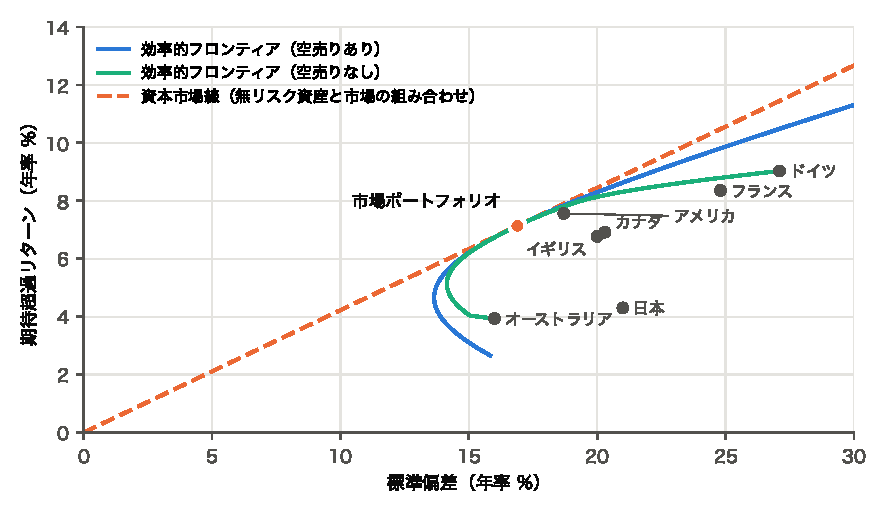
\includegraphics[width=0.94\linewidth]{fig_frontier.pdf}
\caption{G7 で $\Pi$ を期待リターンとしたときの効率的フロンティア。点は各国、オレンジの点は市場ポートフォリオ。}
\label{fig:frontier}
\end{figure}

\section{均衡から少しずらすだけで、比率は大きく動く}\label{sec:sens}

均衡リターンは「何も特別な見方がないとき」の出発点として申し分ない。では、自分の見方を入れるために $\mu$ を少しだけ変えるとどうなるか。\tabref{tab:g7sens} は、全額投資の式~\eqref{eq:mvbudget} で、$\mu$ を変えたときの比率である。

\begin{table}[htbp]
\centering
\caption{G7 で $\mu$ を変えたときの、全額投資の最適比率（\%）。}
\label{tab:g7sens}
\small\tabin{g7_sens}
\end{table}

\begin{itemize}
\item \textbf{ドイツだけ $+1\%$}：ドイツの比率は 5.5\% から \V{sens.gerup}\% に増え、フランスは \V{sens.fraup}\%（空売り）になる。ドイツとフランスの相関は 0.861 と高いので、最適化は「ドイツを買い、フランスを売る」組み合わせを、リスクの小さい儲けとみなす。イギリスも 12.4\% から \V{sens.ukup}\% に減る。ドイツの見方を変えただけなのに、ほかの国の比率が動く。
\item \textbf{ドイツ $+1\%$、フランス $-1\%$}：ドイツは \V{sens.gerfr}\%、フランスは \V{sens.frafr}\% になる。見方としては小さな違いだが、極端な比率になる。
\item \textbf{全部 7\%}：「どの国も同じ」と見たつもりでも、比率は \V{sens.eqmaxname} の \V{sens.eqmax}\% から \V{sens.eqminname} の \V{sens.eqmin}\% まで散らばる。期待リターンを同じにすると、分散が小さく、ほかと相関の低い資産が有利になるからである。
\end{itemize}

ここから分かることは 2 つある。第 1 に、$\mu$ を直接いじるのは危ない。どの資産の $\mu$ を変えても、相関を通してほかの資産の比率まで動く。第 2 に、見方を入れたいなら、「何についての見方か」と「どれくらい自信があるか」を分けて指定し、均衡からのずれをその分だけにとどめる仕組みがほしい。それが次の 2 章で見る BL の仕組みである。

% ============================================================
\chapter{ビューの表し方}\label{ch:views}

BL では、投資家の見方（ビュー）を、次の 3 つに分けて書く。

\begin{enumerate}
\item どの資産の組み合わせについての見方か（行列 $P$）
\item その組み合わせの期待リターンはいくらだと思うか（ベクトル $Q$）
\item その見方はどれくらい確かか（行列 $\Omega$）
\end{enumerate}

\section{絶対的なビューと相対的なビュー}

ビューには 2 つの形がある。

\begin{itemize}
\item \textbf{絶対的なビュー}：「日本株の期待超過リターンは年 6\%」のように、1 つの資産の値を言うもの。
\item \textbf{相対的なビュー}：「ドイツ株はフランス株より年 2\% 高い」のように、資産どうしの差を言うもの。
\end{itemize}

運用の現場の見方は「どちらが勝つか」の形が多く、相対的なビューで書くほうが自然なことが多い。He と Litterman の例は、すべて相対的なビューである。本プロジェクトは、全銘柄について絶対的なビューを置く（\chapref{ch:project}）。

\section{行列 $P$ とベクトル $Q$}

$K$ 個のビューを、まとめて次のように書く。
\begin{equation}
P\mu = Q + \varepsilon
\label{eq:view}
\end{equation}
$P$ の $k$ 行目 $p_k$ は、ビュー $k$ が対象にする「ポートフォリオ」（各資産の重み）である。$p_k\mu$ はそのポートフォリオの期待リターンで、$Q_k$ はそれについての投資家の予想値である。$\varepsilon$ は予想の誤差で、次の節で扱う。

\begin{itemize}
\item 絶対的なビューの行は、その資産のところだけ 1 で、ほかは 0 である。
\item 相対的なビューの行は、買う側の重みの合計が 1、売る側の重みの合計が $-1$ で、行の合計は 0 になる。
\end{itemize}

\begin{exbox}[計算例 3.1：He と Litterman のビュー]
\textbf{ビュー 1}：ドイツの株式は、ほかのヨーロッパ（フランスとイギリス）を年 5\% 上回る。

「ほかのヨーロッパ」は、時価総額の比率で重み付けする。フランスは $5.2/(5.2+12.4) = 0.2955$、イギリスは $12.4/(5.2+12.4) = 0.7045$ である。

\textbf{ビュー 2}：カナダの株式は、アメリカの株式を年 3\% 上回る。

国の順番を（オーストラリア、カナダ、フランス、ドイツ、日本、イギリス、アメリカ）とすると
\[
P = \begin{pmatrix}
0 & 0 & \V{ex1.pFRA} & 1 & 0 & \V{ex1.pUK} & 0 \\
0 & 1 & 0 & 0 & 0 & 0 & -1
\end{pmatrix},\qquad
Q = \begin{pmatrix} 0.05 \\ 0.03 \end{pmatrix}.
\]
どちらの行も合計は 0 である。
\end{exbox}

\section{均衡が示すビューの値}\label{sec:impliedview}

ビューのポートフォリオ $p_k$ についても、均衡が示す期待リターン $p_k\Pi$ を計算できる。これと $Q_k$ を比べると、そのビューが均衡に比べてどれだけ強気かが分かる。

\begin{exbox}[計算例 3.2：均衡が示すビューの値]
ビュー 1 では
\[
p_1\Pi = 9.03\% - 0.2955 \times 8.36\% - 0.7045 \times 6.77\% = \V{ex1.pPi}\%
\]
である。市場は、ドイツがほかのヨーロッパを年 \V{ex1.pPi}\% 上回ると見ている。投資家の $Q_1 = 5\%$ は、それより \V{ex1.gap}\% 強気である。

ビュー 2 では $p_2\Pi = 6.92\% - 7.56\% = \V{ex2.p2Pi}\%$ で、市場はカナダがアメリカを下回ると見ている。$Q_2 = 3\%$ は \V{ex2.gap2}\% 強気である。
\end{exbox}

後で見るとおり、BL で効くのは $Q$ の値そのものではなく、均衡との差 $Q - P\Pi$ である。$Q = P\Pi$ のビューは、期待リターンについて新しい情報を何も持たない。

\section{ビューの不確かさ $\Omega$}

式~\eqref{eq:view} の誤差 $\varepsilon$ は、平均 0、共分散 $\Omega$ の正規分布に従うとする。
\begin{equation}
\varepsilon \sim \mathcal{N}(0,\ \Omega)
\end{equation}
ふつうは、ビューどうしの誤差は独立だとして、$\Omega$ を対角行列 $\diag(\omega_1, \dots, \omega_K)$ にする。$\omega_k$ が小さいほど、ビュー $k$ に自信があることを表す。

$\omega_k$ をどう決めるかは、BL を使ううえで最も悩ましい点である。He と Litterman は、次のように置いた。
\begin{equation}
\omega_k = p_k\,(\tau\Sigma)\,p_k\T
\label{eq:omegahl}
\end{equation}
右辺は、事前の見方（次の章の $\mu \sim \mathcal{N}(\Pi, \tau\Sigma)$）のもとでの $p_k\mu$ の分散である。つまり、「ビューの値の不確かさは、均衡がそのポートフォリオについて持つ不確かさと同じ」とする置き方である。次の章で見るとおり、こうするとビューと均衡が同じ重みで混ざる。

\begin{exbox}[計算例 3.3：ビュー 1 の不確かさ]
ビュー 1 のポートフォリオの分散は $p_1\Sigma p_1\T = \V{ex1.pSp}$（標準偏差 14.6\%）である。$\tau = 0.05$ とすると
\[
\omega_1 = 0.05 \times \V{ex1.pSp} = \V{ex1.omega}
\]
で、標準偏差は $\sqrt{\V{ex1.omega}} = \V{ex1.viewsd}\%$ である。ビュー 1 は「ドイツはほかのヨーロッパを $5\% \pm \V{ex1.viewsd}\%$ 上回る」と言っていることになる。同じように、ビュー 2 は $\omega_2 = \V{ex2.omegaB}$ である。
\end{exbox}

ほかの決め方には、次のものがある。

\begin{center}
\small
\begin{tabular}{p{4.0cm}p{9.2cm}}
\toprule
決め方 & 内容 \\
\midrule
均衡に合わせる（He と Litterman） & 式~\eqref{eq:omegahl}。ビューと均衡を同じ重みで扱う \\
自信の度合いから逆算する（Idzorek） & ビューごとに「何 \% 自信があるか」を決め、それに合う $\omega_k$ を逆算する \\
過去の当たり具合から決める & 過去の予想が実際にどれだけ外れたか（予測誤差の分散）を使う \\
回答のばらつきを使う（本プロジェクト） & LLM に同じ質問を 30 回行い、回答の分散を $\omega_k$ にする \\
\bottomrule
\end{tabular}
\end{center}

\section{$\tau$ の意味}

次の章では、真の期待リターン $\mu$ を確率変数とみなし、その事前の分布を $\mathcal{N}(\Pi, \tau\Sigma)$ とする。ここに出てくる 2 つの共分散を区別しておく。

\begin{itemize}
\item $\Sigma$：リターン $r$ そのもののぶれ。来年の株価が上がるか下がるか。
\item $\tau\Sigma$：期待リターン $\mu$ についての不確かさ。平均的にはどれくらい上がるはずか、を私たちがどれだけ知らないか。
\end{itemize}

平均を $T$ 個の独立な観測から推定すれば、その推定値の共分散は $\Sigma/T$ である。この見方では $\tau \approx 1/T$ で、$\tau = 0.05$ は 20 年分、$\tau = 0.025$ は 40 年分の年次データで平均を推定したのと同じ確かさに当たる。実際には 0.01〜0.05 程度の値がよく使われる。He と Litterman は $\tau = 0.05$、本プロジェクトの元論文と本プロジェクトは $\tau = 0.025$ である。

たとえば $\tau = 0.05$ のとき、ドイツの期待リターンの事前の標準偏差は $\sqrt{0.05} \times 27.1\% = 6.06\%$ である。事前の見方は「ドイツの期待リターンは $9.03\% \pm 6.06\%$」となる。

% ============================================================
\chapter{ベイズで混ぜる：Black-Litterman の公式}\label{ch:bl}

\section{2 段の確率モデル}

BL は、真の期待リターン $\mu$ を分からない量として扱い、次のモデルを考える。
\begin{align}
r \mid \mu &\sim \mathcal{N}(\mu,\ \Sigma) && \text{リターンは、期待リターンのまわりにぶれる} \label{eq:model1}\\
\mu &\sim \mathcal{N}(\Pi,\ \tau\Sigma) && \text{事前の見方：期待リターンは均衡のまわりにある} \label{eq:prior}\\
Q \mid \mu &\sim \mathcal{N}(P\mu,\ \Omega) && \text{ビュー：$P\mu$ についての誤差のある予想} \label{eq:likelihood}
\end{align}
式~\eqref{eq:likelihood} は、式~\eqref{eq:view} を書き直したものである。$Q$ を「$P\mu$ を誤差つきで観測したデータ」とみなし、ベイズの定理で $\mu$ の分布を更新する。Black と Litterman の原論文は、この組み合わせを Theil の混合推定（標本の情報と事前の情報をまとめて推定する方法）として説明していた。ベイズの事前分布と事後分布として読む説明は、その後に広まった（Satchell and Scowcroft 2000 など）。どちらで読んでも、得られる式は同じである。

\section{1 資産・1 ビューの場合}\label{sec:scalar}

まず、資産が 1 つで、その期待リターンについて絶対的なビューを 1 つ持つ場合を考える。事前は $\mu \sim \mathcal{N}(\Pi, \tau\sigma^2)$、ビューは $Q \mid \mu \sim \mathcal{N}(\mu, \omega)$ である。ベイズの定理から、事後の密度は事前の密度と尤度の積に比例する。
\[
p(\mu \mid Q) \propto
\exp\!\left(-\frac{(\mu - \Pi)^2}{2\tau\sigma^2}\right)
\exp\!\left(-\frac{(Q - \mu)^2}{2\omega}\right)
\]
指数の部分を $\mu$ について整理する（平方完成）。
\[
-\frac{1}{2}\left[\left(\frac{1}{\tau\sigma^2} + \frac{1}{\omega}\right)\mu^2 - 2\left(\frac{\Pi}{\tau\sigma^2} + \frac{Q}{\omega}\right)\mu\right] + \text{定数}
= -\frac{1}{2}\cdot\frac{(\mu - \mub)^2}{v} + \text{定数}
\]
ここで
\begin{equation}
\frac{1}{v} = \frac{1}{\tau\sigma^2} + \frac{1}{\omega},\qquad
\mub = v\left(\frac{\Pi}{\tau\sigma^2} + \frac{Q}{\omega}\right)
\label{eq:scalarpost}
\end{equation}
である。事後の分布も正規分布 $\mathcal{N}(\mub, v)$ になる。分散の逆数を精度と呼ぶと、式~\eqref{eq:scalarpost} は次のように読める。

\begin{itemize}
\item 事後の精度は、事前の精度とビューの精度の和である。情報が増えるので、事後の分散はどちらよりも小さい。
\item 事後の平均は、$\Pi$ と $Q$ を、それぞれの精度で重み付けした平均である。
\end{itemize}

事後の平均は、さらに次の形に書き直せる。
\begin{equation}
\mub = \Pi + k\,(Q - \Pi),\qquad k = \frac{\tau\sigma^2}{\tau\sigma^2 + \omega}
\label{eq:adoption}
\end{equation}
$k$ は、均衡から見たビューの「驚き」$Q - \Pi$ のうち、何割を受け入れるかを表す。この資料では $k$ を\textbf{採用率}と呼ぶ。採用率は 2 つの不確かさの比 $\omega/(\tau\sigma^2)$ だけで決まる（\figref{fig:adoption}）。

\begin{exbox}[計算例 4.1：1 資産の更新]
$\Pi = \V{sc.pi}\%$、$\sigma = \V{sc.sig}\%$、$\tau = \V{sc.tau}$ とする。事前の分散は $\tau\sigma^2 = 0.05 \times 0.04 = \V{sc.ts}$（標準偏差 \V{sc.tssd}\%）である。ビューは $Q = \V{sc.q}\%$ とする。

He と Litterman の置き方では $\omega = \tau\sigma^2 = \V{sc.ts}$ なので、$k = 0.002/(0.002 + 0.002) = 0.5$、$\mub = 5\% + 0.5 \times (10\% - 5\%) = \V{sc.post}\%$ である。事後の分散は $1/(1/0.002 + 1/0.002) = 0.001$ で、標準偏差は \V{sc.postsd}\% に減る（\figref{fig:scalar}）。$\omega$ を変えたときの結果を\tabref{tab:scalar}に示す。
\end{exbox}

\begin{figure}[htbp]
\centering
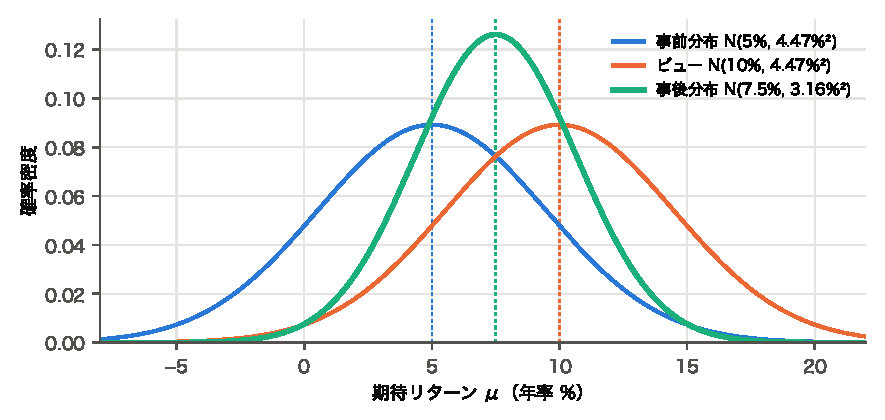
\includegraphics[width=0.94\linewidth]{fig_scalar.pdf}
\caption{計算例 4.1 の事前分布、ビュー、事後分布。事後分布は 2 つの間にあり、幅が狭い。}
\label{fig:scalar}
\end{figure}

\begin{table}[htbp]
\centering
\caption{ビューの不確かさ $\omega$ と事後の期待リターン（$\Pi = 5\%$、$Q = 10\%$、$\tau\sigma^2 = 0.002$）。}
\label{tab:scalar}
\small\tabin{scalar}
\end{table}

\begin{figure}[htbp]
\centering
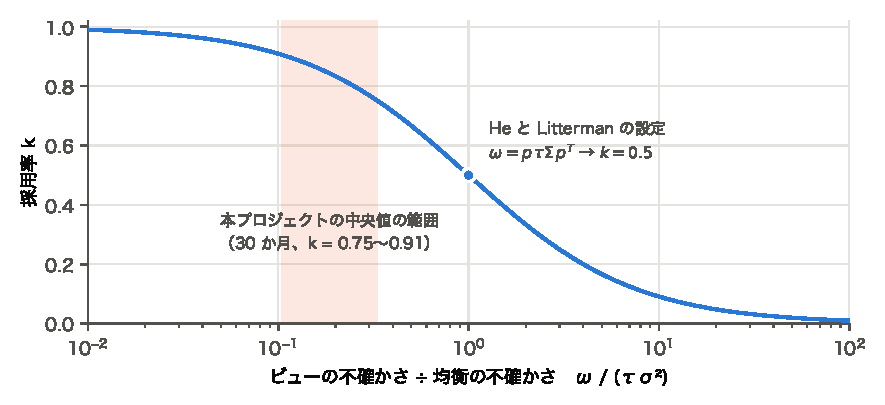
\includegraphics[width=0.94\linewidth]{fig_adoption.pdf}
\caption{採用率 $k$ と、2 つの不確かさの比 $\omega/(\tau\sigma^2)$ の関係。He と Litterman の置き方は $k = 0.5$。網かけは、本プロジェクトの 30 か月の判断日それぞれで、全銘柄の比の中央値を取ったときの範囲（\chapref{ch:project}）。}
\label{fig:adoption}
\end{figure}

\section{一般の場合の導出}

$N$ 資産・$K$ ビューの場合も、やることは同じである。事後の密度の対数は、定数を除いて
\[
\log p(\mu \mid Q) = -\frac{1}{2}(\mu - \Pi)\T(\tau\Sigma)^{-1}(\mu - \Pi) - \frac{1}{2}(Q - P\mu)\T\Omega^{-1}(Q - P\mu) + \text{定数}
\]
である。$\mu$ の 2 次の項と 1 次の項を集めると
\[
= -\frac{1}{2}\left[\mu\T H\mu - 2\mu\T h\right] + \text{定数},\qquad
H = (\tau\Sigma)^{-1} + P\T\Omega^{-1}P,\quad
h = (\tau\Sigma)^{-1}\Pi + P\T\Omega^{-1}Q
\]
となる。$H$ は対称なので、平方完成すると $-\frac{1}{2}(\mu - H^{-1}h)\T H(\mu - H^{-1}h) + \text{定数}$ である。したがって、事後の分布は
\begin{equation}
\mu \mid Q \sim \mathcal{N}(\mub,\ M),\qquad
\mub = H^{-1}h,\quad M = H^{-1}
\end{equation}
で、書き下すと次の BL の公式になる。

\begin{thmbox}[Black-Litterman の公式（情報形）]
\begin{align}
\mub &= \left[(\tau\Sigma)^{-1} + P\T\Omega^{-1}P\right]^{-1}\left[(\tau\Sigma)^{-1}\Pi + P\T\Omega^{-1}Q\right] \label{eq:blinfo}\\
M &= \left[(\tau\Sigma)^{-1} + P\T\Omega^{-1}P\right]^{-1} \label{eq:blM}
\end{align}
\end{thmbox}

1 資産のときと同じく、事後の精度 $H$ は事前の精度 $(\tau\Sigma)^{-1}$ とビューの精度 $P\T\Omega^{-1}P$ の和で、事後の平均はそれぞれの精度で重み付けした平均である。

\section{もう 1 つの形：更新形}\label{sec:update}

式~\eqref{eq:blinfo} は、$N \times N$ の逆行列を 3 回使う。$\Omega$ の逆行列も要るので、ビューの不確かさが 0（完全な自信）のときは使えない。同じ式は、次の形にも書ける。

\begin{thmbox}[Black-Litterman の公式（更新形）]
\begin{align}
\mub &= \Pi + \tau\Sigma P\T\left(P\tau\Sigma P\T + \Omega\right)^{-1}\left(Q - P\Pi\right) \label{eq:blupdate}\\
M &= \tau\Sigma - \tau\Sigma P\T\left(P\tau\Sigma P\T + \Omega\right)^{-1}P\tau\Sigma \label{eq:blMupdate}
\end{align}
\end{thmbox}

逆行列は $K \times K$ の 1 つだけで、$\Omega$ が特異でもかまわない。式~\eqref{eq:adoption} の 1 資産の形を、そのまま行列にしたものになっている。

\paragraph{同じであることの確かめ}
$A = \tau\Sigma$、$G = PAP\T + \Omega$ とおく。Woodbury の公式（付録 A）から
\[
M = (A^{-1} + P\T\Omega^{-1}P)^{-1} = A - AP\T G^{-1}PA
\]
で、式~\eqref{eq:blMupdate} が出る。これを $h = A^{-1}\Pi + P\T\Omega^{-1}Q$ に掛けると
\[
\mub = Mh = \Pi + AP\T\Omega^{-1}Q - AP\T G^{-1}P\Pi - AP\T G^{-1}(PAP\T)\Omega^{-1}Q
\]
である。最後の項で $PAP\T = G - \Omega$ を使うと、$AP\T G^{-1}(G - \Omega)\Omega^{-1}Q = AP\T\Omega^{-1}Q - AP\T G^{-1}Q$ なので、
\[
\mub = \Pi - AP\T G^{-1}P\Pi + AP\T G^{-1}Q = \Pi + AP\T G^{-1}(Q - P\Pi)
\]
となり、式~\eqref{eq:blupdate} が出る。付録 A では、$(\mu, Q)$ の同時分布から条件付き分布を求める、別の導き方も示す。

\begin{keybox}[本プロジェクトのコードとの対応]
本プロジェクトの \code{blm/black\_litterman.py} には、2 つの関数がある。\code{posterior\_returns} は更新形~\eqref{eq:blupdate}、\code{posterior\_returns\_original} は元の実装と同じ情報形~\eqref{eq:blinfo}（逆行列の代わりに疑似逆行列）で計算する。数学的には同じだが、$\Omega$ に 0 が含まれるときに結果が変わる（\secref{sec:pinv}）。
\end{keybox}

\section{更新形の読み方：ビューの驚きが、相関を通じて広がる}

式~\eqref{eq:blupdate} を、ビューが 1 つ（$K = 1$、$P = p$）の場合に書くと
\begin{equation}
\mub = \Pi + g\,(Q - p\Pi),\qquad
g = \frac{\tau\Sigma p\T}{p\tau\Sigma p\T + \omega}
\label{eq:gain}
\end{equation}
である。$Q - p\Pi$ は「ビューが均衡に比べてどれだけ強気か」（驚き）、$g$ はその驚きを各資産に配る係数である。$g$ の $i$ 番目の成分は、$\tau\,\mathrm{Cov}(r_i,\ p\,r)$、つまり資産 $i$ とビューのポートフォリオの共分散に比例する。ビューに出てこない資産も、ビューのポートフォリオと相関があれば、期待リターンが動く。

\begin{exbox}[計算例 4.2：G7 の例 1 を手で計算する]
ビュー 1 だけを持つ場合（$\tau = 0.05$、$\omega_1 = p_1\tau\Sigma p_1\T$）を計算する。

\textbf{手順 1（驚き）}：計算例 3.2 から $p_1\Pi = \V{ex1.pPi}\%$、$Q_1 - p_1\Pi = \V{ex1.gap}\%$。

\textbf{手順 2（分母）}：$p_1\tau\Sigma p_1\T = \V{ex1.ptSp}$、$\omega_1 = \V{ex1.omega}$ なので、分母は $2 \times \V{ex1.ptSp}$。

\textbf{手順 3（配る係数）}：$\tau\Sigma p_1\T$ を計算し、分母で割る（\tabref{tab:ex1steps}）。

\textbf{手順 4（足す）}：$\mub_i = \Pi_i + g_i \times \V{ex1.gap}\%$。

確かめ：ビューのポートフォリオの事後の値は
$p_1\mub = p_1\Pi + \dfrac{p_1\tau\Sigma p_1\T}{p_1\tau\Sigma p_1\T + \omega_1}(Q_1 - p_1\Pi) = \V{ex1.pPi}\% + 0.5 \times \V{ex1.gap}\% = \V{ex1.pmu}\%$ で、均衡の \V{ex1.pPi}\% とビューの 5\% のちょうど中間になる。式~\eqref{eq:omegahl} の置き方では、採用率が 0.5 になるからである。
\end{exbox}

\begin{table}[htbp]
\centering
\caption{例 1 の事後の期待リターンの計算（年率）。$g_i$ は式~\eqref{eq:gain} の係数。}
\label{tab:ex1steps}
\small\tabin{ex1_steps}
\end{table}

\tabref{tab:ex1steps} を見ると、ドイツだけでなく、7 か国すべての期待リターンが上がっている。ドイツはどの国とも正の相関を持つので、「ドイツが思ったより強い」という情報は、ほかの国にも少しずつ良い知らせになる。フランスとイギリスも上がるのは、ドイツとの相関が高いからである。ただし、上がり方はドイツより小さいので、ドイツとほかのヨーロッパの差は広がる。

\section{事後の不確かさと、予測の共分散}

事後の共分散 $M$ は、ビューを知った後の $\mu$ の不確かさである。ビューがなければ $M = \tau\Sigma$ で、ビューがあると式~\eqref{eq:blMupdate} の第 2 項の分だけ小さくなる。

最適化で使うのは、$\mu$ ではなく、来期のリターン $r$ の予測の分布である。式~\eqref{eq:model1} から $r = \mu + e$（$e \sim \mathcal{N}(0, \Sigma)$、$\mu$ と独立）と書けるので
\begin{equation}
r \mid Q \sim \mathcal{N}(\mub,\ \Sigma + M) = \mathcal{N}(\mub,\ \Sp)
\label{eq:predictive}
\end{equation}
である。リターンのぶれ $\Sigma$ に、期待リターンが分からないことによるぶれ $M$ が加わる。ビューがないときは $\Sp = (1 + \tau)\Sigma$ である。

\begin{table}[htbp]
\centering
\caption{例 1 の不確かさ（標準偏差、年率 \%）。ビューで $\mu$ の不確かさは減るが、$\Sigma + M$ に対しては小さな違いである。}
\label{tab:ex1unc}
\small\tabin{ex1_unc}
\end{table}

\tabref{tab:ex1unc} では、ドイツの期待リターンの不確かさが、ビューによって事前の \V{ex1.Mratio} 倍に減っている。一方、リターンそのもののぶれ $\Sigma$ に比べると $M$ は小さく、$\Sigma + M$ は $\Sigma$ とほとんど変わらない。

\section{極端な場合}

式~\eqref{eq:blupdate} で、いくつかの極端な場合を確かめておく。

\begin{itemize}
\item \textbf{ビューがない}：$\mub = \Pi$、$M = \tau\Sigma$。
\item \textbf{ビューに自信がない}（$\Omega \to \infty$）：$(P\tau\Sigma P\T + \Omega)^{-1} \to 0$ なので $\mub \to \Pi$。ビューは無視される。
\item \textbf{ビューに完全な自信がある}（$\Omega \to 0$）：$\mub = \Pi + \tau\Sigma P\T(P\tau\Sigma P\T)^{-1}(Q - P\Pi)$。左から $P$ を掛けると $P\mub = Q$ で、ビューがそのまま成り立つ。ビューに出てこない方向は、均衡からの「最小の変更」で調整される。
\item \textbf{ビューが均衡と同じ}（$Q = P\Pi$）：$\mub = \Pi$。期待リターンは変わらない。ただし $M$ は小さくなる。
\item \textbf{$\tau$ と $\Omega$ を同じ倍率で変える}：$\tau\Sigma$ と $\Omega$ を両方 $c$ 倍しても、式~\eqref{eq:blupdate} の $\mub$ は変わらない。$\mub$ を決めるのは 2 つの比である（\secref{sec:tau}）。
\end{itemize}

% ============================================================
\chapter{He と Litterman の主結果：最適ポートフォリオの形}\label{ch:hl}

前の章で、ビューを入れた期待リターン $\mub$ が求まった。He と Litterman の論文の中心は、それを最適化に入れたときに、どんな比率が出てくるかの分析である。

\section{制約のない最適化}

予測の分布~\eqref{eq:predictive} を使い、式~\eqref{eq:utility} の効用を最大にする。制約を付けなければ、式~\eqref{eq:mvfree} と同じく
\begin{equation}
w^* = (\delta\Sp)^{-1}\mub,\qquad \Sp = \Sigma + M
\label{eq:wstar}
\end{equation}
である。

\paragraph{ビューがないとき}
$\mub = \Pi = \delta\Sigma\weq$、$\Sp = (1 + \tau)\Sigma$ なので
\begin{equation}
w^* = \frac{1}{\delta(1 + \tau)}\Sigma^{-1}\,\delta\Sigma\weq = \frac{\weq}{1 + \tau}
\end{equation}
となる。ビューがなければ、市場の比率をそのまま $1/(1 + \tau)$ 倍に縮めたものを持つ。期待リターンが分からない分だけリスクが大きく見えるので、少しだけリスク資産を減らし、残りを無リスク資産に置く。$\tau = 0.05$ なら $1/1.05 = 95.2\%$ である。

\section{主結果：市場ポートフォリオとビューのポートフォリオの和}

\begin{thmbox}[He と Litterman の結果]
制約のない BL の最適比率は
\begin{equation}
w^* = \frac{1}{1 + \tau}\left(\weq + P\T\Lambda\right)
\label{eq:hl}
\end{equation}
と書ける。$\Lambda$ は $K$ 次元のベクトルで、
\begin{equation}
\Lambda = \frac{\tau\Omega^{-1}Q}{\delta} - \frac{A^{-1}P\Sigma\weq}{1 + \tau} - \frac{A^{-1}P\Sigma P\T}{1 + \tau}\cdot\frac{\tau\Omega^{-1}Q}{\delta},\qquad
A = \frac{\Omega}{\tau} + \frac{P\Sigma P\T}{1 + \tau}
\label{eq:lambda}
\end{equation}
である。
\end{thmbox}

$P\T\Lambda = \sum_k \lambda_k\,p_k\T$ は、ビューのポートフォリオ $p_k$ を重み $\lambda_k$ で足したものである。つまり、BL の最適比率は「市場の比率」に「ビューのポートフォリオ」を足し、全体を $1/(1+\tau)$ 倍したものになる。\textbf{ビューに出てこない資産の比率は、市場の比率（の $1/(1+\tau)$ 倍）から動かない。}第 2 章で見た平均分散最適化の、どこを変えても全部が動く性質とは、対照的である。

\subsection{$\Lambda$ を整理する}

式~\eqref{eq:lambda} の 3 つの項は、まとめると簡単になる。$(1 + \tau)A = (1 + \tau)\Omega/\tau + P\Sigma P\T$ だから
\[
\frac{P\Sigma P\T}{1 + \tau}\cdot\tau\Omega^{-1} = \left(A - \frac{\Omega}{\tau}\right)\tau\Omega^{-1} = A\tau\Omega^{-1} - I
\]
である。これを第 3 項に使うと、第 1 項と打ち消し合って $A^{-1}Q/\delta$ が残る。第 2 項は $P\Sigma\weq = P\Pi/\delta$ と書けるので、
\begin{equation}
\Lambda = \frac{1}{\delta}A^{-1}\left(Q - \frac{P\Pi}{1 + \tau}\right),\qquad
A = \frac{\Omega}{\tau} + \frac{P\Sigma P\T}{1 + \tau}
\label{eq:lambdasimple}
\end{equation}
となる。この資料の計算では、2 つの形が一致することを数値でも確かめている。

\subsection{導き方}

式~\eqref{eq:hl} と式~\eqref{eq:lambdasimple} が式~\eqref{eq:wstar} と一致することを確かめる。示すべきことは
\[
\delta\Sp\,\frac{\weq + P\T\Lambda}{1 + \tau} = \mub
\]
である。$G = P\tau\Sigma P\T + \Omega$ とおくと、式~\eqref{eq:blMupdate} から
\[
\Sp = \Sigma + M = (1 + \tau)\Sigma - \tau\Sigma P\T G^{-1}P\tau\Sigma .
\]

\textbf{市場の部分}：$\delta\Sigma\weq = \Pi$ を使うと
\[
\delta\Sp\weq = (1 + \tau)\Pi - \tau\Sigma P\T G^{-1}\,\tau P\Pi .
\]

\textbf{ビューの部分}：
\[
\delta\Sp P\T\Lambda = \delta\,\tau\Sigma P\T\left[\frac{1 + \tau}{\tau}I - G^{-1}\tau P\Sigma P\T\right]\Lambda .
\]
$\tau P\Sigma P\T = G - \Omega$ だから、かっこの中は
\[
\frac{1 + \tau}{\tau}I - I + G^{-1}\Omega = G^{-1}\left(\frac{G}{\tau} + \Omega\right)
= G^{-1}\left(P\Sigma P\T + \frac{1 + \tau}{\tau}\Omega\right) = (1 + \tau)\,G^{-1}A
\]
となる。よって $\delta\Sp P\T\Lambda = (1 + \tau)\,\tau\Sigma P\T G^{-1}\,\delta A\Lambda$ である。

\textbf{合わせる}：2 つを足して $1 + \tau$ で割ると
\[
\delta\Sp\,\frac{\weq + P\T\Lambda}{1 + \tau}
= \Pi + \tau\Sigma P\T G^{-1}\left(\delta A\Lambda - \frac{\tau P\Pi}{1 + \tau}\right).
\]
これが式~\eqref{eq:blupdate} の $\mub = \Pi + \tau\Sigma P\T G^{-1}(Q - P\Pi)$ に等しくなる条件は
\[
\delta A\Lambda - \frac{\tau P\Pi}{1 + \tau} = Q - P\Pi
\quad\Longleftrightarrow\quad
\delta A\Lambda = Q - \frac{P\Pi}{1 + \tau}
\]
で、これは式~\eqref{eq:lambdasimple} そのものである。\hfill$\square$

\section{4 つの性質}

He と Litterman は、この形から BL の比率の性質を読み取っている。要約すると次の 4 つである。

\begin{thmbox}[BL の最適比率の性質（He と Litterman）]
\begin{enumerate}
\item 制約のない最適比率は、市場の比率に、ビューを表すポートフォリオの重み付きの和を足したもの（を $1/(1+\tau)$ 倍したもの）である。
\item ビューのポートフォリオの重み $\lambda_k$ は、そのビューが「均衡とほかのビューから示される値」より強気なら正になる。
\item ビューを強気にするほど、重み $\lambda_k$ は大きくなる。
\item ビューへの自信が強いほど（$\omega_k$ が小さいほど）、重みの大きさ $|\lambda_k|$ は大きくなる。
\end{enumerate}
\end{thmbox}

ビューが 1 つのときは、式~\eqref{eq:lambdasimple} がスカラーの式になるので、性質 2〜4 がすぐに確かめられる。
\begin{equation}
\lambda = \frac{Q - p\Pi/(1 + \tau)}{\delta\left(\omega/\tau + p\Sigma p\T/(1 + \tau)\right)}
\label{eq:lambdaone}
\end{equation}
\begin{itemize}
\item 分母は正なので、$\lambda > 0$ となるのは $Q > p\Pi/(1 + \tau)$ のときである（性質 2）。
\item $\lambda$ は $Q$ について増加する（性質 3）。
\item $\omega$ が小さいほど分母が小さくなり、$|\lambda|$ は大きくなる（性質 4）。
\end{itemize}

境目が $p\Pi$ ではなく $p\Pi/(1 + \tau)$ になっているのは、式~\eqref{eq:hl} で市場の比率そのものが $1/(1 + \tau)$ 倍されているためである。$Q = p\Pi$（期待リターンは何も変えないビュー）でも、そのビューによって $p\mu$ の不確かさが減るので、そのポートフォリオを少しだけ多く持つ。例 1 では、$Q_1 = p_1\Pi$ のとき $\lambda_1 = \V{ex1.lamAtpPi}$ で、ほぼ 0 である。

ビューが複数あるときは、$A^{-1}$ がビューどうしの関係を調整する。$A$ の非対角成分 $p_j\Sigma p_k\T/(1 + \tau)$ は、ビューのポートフォリオどうしの共分散である。似たポートフォリオのビューが 2 つあれば、一方のビューの情報は他方のビューの重みにも影響する。性質 2 の「ほかのビューから示される値」は、このことを指している。

ビューがすべて相対的なビュー（$P\one = 0$）なら、$\one\T P\T\Lambda = 0$ なので、比率の合計は $\one\T w^* = 1/(1 + \tau)$ のまま変わらない。相対的なビューは、リスク資産全体の量を変えずに、中身の配分だけを変える。

\section{例 1：ドイツとほかのヨーロッパ}

ビュー 1 だけを持つ場合の結果を\tabref{tab:ex1}に示す。

\begin{table}[htbp]
\centering
\caption{例 1：ドイツがほかのヨーロッパを 5\% 上回る（年率 \%、$\tau = 0.05$、$\delta = 2.5$）。}
\label{tab:ex1}
\small\tabin{ex1}
\end{table}

\begin{exbox}[計算例 5.1：$\lambda_1$ を手で計算する]
式~\eqref{eq:lambdaone} に入れる。
\begin{align*}
\frac{\omega_1}{\tau} &= \frac{\V{ex1.omega}}{0.05} = \V{ex1.omtau}, \qquad
\frac{p_1\Sigma p_1\T}{1 + \tau} = \frac{\V{ex1.pSp}}{1.05} = \V{ex1.pSptau}, \qquad
A = \V{ex1.A}, \\
Q_1 - \frac{p_1\Pi}{1 + \tau} &= 5\% - \frac{\V{ex1.pPi}\%}{1.05} = \V{ex1.d}\%, \qquad
\lambda_1 = \frac{\V{ex1.d}\%}{2.5 \times \V{ex1.A}} = \V{ex1.lam}.
\end{align*}
比率の変化は $w^* - \weq/(1 + \tau) = \lambda_1 p_1\T/(1 + \tau)$ で、ドイツが $+\V{ex1.lamscaled} = +30.2\%$、フランスが $\V{ex1.lamscaled} \times (\V{ex1.pFRA}) = -8.9\%$、イギリスが $\V{ex1.lamscaled} \times (\V{ex1.pUK}) = -21.3\%$ である。\tabref{tab:ex1} の最後の列と一致する。
\end{exbox}

\tabref{tab:ex1} で注目すべき点は 2 つある。

第 1 に、期待リターン $\mub$ は 7 か国すべてで変わったのに、比率が $\weq/(1 + \tau)$ から動いたのは、ビューに出てくるドイツ、フランス、イギリスの 3 か国だけである。ほかの国の期待リターンの上昇は、ドイツとの相関から「当然そうなるはずの分」で、比率を変える理由にはならない。平均分散最適化に $\mub$ を入れて比率がおかしくならないのは、$\mub$ が $\Sigma$ と整合するように作られているからである。

第 2 に、比率の変化は「ドイツを買い、ほかのヨーロッパを時価総額の比で売る」ビューのポートフォリオの形をしている。投資家は、自分のビューがそのまま比率に表れるので、結果を説明しやすい。He と Litterman が「直観的」と呼んだのは、この性質である。

\section{例 2：カナダとアメリカのビューを足す}

ビュー 2（カナダがアメリカを 3\% 上回る）を足した結果を\tabref{tab:ex2}と\figref{fig:ex2}に示す。

\begin{table}[htbp]
\centering
\caption{例 2：ビュー 1 とビュー 2（年率 \%）。}
\label{tab:ex2}
\small\tabin{ex2}
\end{table}

\begin{figure}[htbp]
\centering
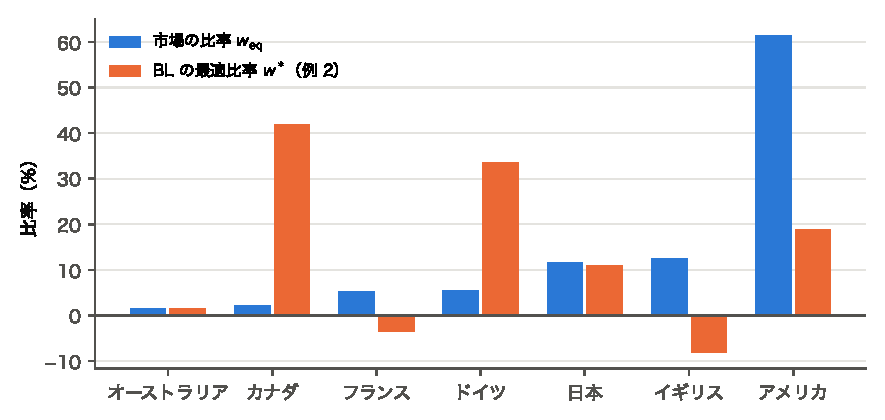
\includegraphics[width=0.94\linewidth]{fig_ex2_weights.pdf}
\caption{例 2 の市場の比率と BL の最適比率。動くのはビューに出てくる 5 か国だけ。}
\label{fig:ex2}
\end{figure}

重みは $\lambda_1 = \V{ex2.lamA}$、$\lambda_2 = \V{ex2.lamB}$ である。カナダは \V{ex2.CAN}\%、アメリカは \V{ex2.USA}\% になる。ビュー 2 の驚き（\V{ex2.gap2}\%）はビュー 1（\V{ex1.gap}\%）と同じくらいだが、ビュー 2 のポートフォリオは分散が小さい（$\omega_2 < \omega_1$）ので、重みが大きい。

$\lambda_1$ は、例 1 の \V{ex1.lam} から \V{ex2.lamA} に少し下がっている。2 つのビューのポートフォリオの相関は \V{ex2.viewcorr} で、わずかに正である。ビュー 2 の情報の一部は、ビュー 1 の方向にも効くので、その分だけビュー 1 に頼る必要が減る。比率の合計は、例 1 と同じ \V{ex2.wsum}\%（$= 1/1.05$）である。どちらも相対的なビューだからである。

\section{例 3：ビューを強気にする}

ビュー 2 を 3\% から 4\% に強めると（\tabref{tab:ex3}）、$\lambda_2$ は \V{ex2.lamB} から \V{ex3.lamB} に増える（性質 3）。$\lambda_1$ は \V{ex2.lamA} から \V{ex3.lamA} に、わずかに動く。

\begin{table}[htbp]
\centering
\caption{例 3：ビュー 2 を 4\% に強めたとき（年率 \%）。}
\label{tab:ex3}
\small\tabin{ex3}
\end{table}

\section{例 4：ビューへの自信を下げる}

例 3 から、ビュー 1 の不確かさ $\omega_1$ を 2 倍にする（\tabref{tab:ex4}）。$\lambda_1$ は \V{ex3.lamA} から \V{ex4.lamA} に下がる（性質 4）。ビュー 1 の事後の値 $p_1\mub$ も \V{ex3.p1mu}\% から \V{ex4.p1mu}\% に下がり、均衡の値（\V{ex1.pPi}\%）に近づく。

\begin{table}[htbp]
\centering
\caption{例 4：例 3 で、ビュー 1 の $\omega_1$ を 2 倍にしたとき（年率 \%）。}
\label{tab:ex4}
\small\tabin{ex4}
\end{table}

\section{例 5：重みが 0 になるビュー}

最後に、ビュー 1 を 5\% のまま、ビュー 2 の重みがちょうど 0 になる $Q_2$ を求める。式~\eqref{eq:lambdasimple} は $Q$ について 1 次式なので、$\lambda_2 = 0$ は $Q_2$ の 1 次方程式になり、解は $Q_2 = \V{ex5.qstar}\%$ である（\tabref{tab:ex5}）。このときカナダとアメリカの比率は、市場の比率の $1/(1 + \tau)$ 倍のままになる。

\begin{table}[htbp]
\centering
\caption{例 5：ビュー 2 の重みが 0 になる $Q_2$（年率 \%）。}
\label{tab:ex5}
\small\tabin{ex5}
\end{table}

この値は、均衡の値 $p_2\Pi = \V{ex5.p2Pi}\%$ でも、$p_2\Pi/(1 + \tau) = \V{ex5.p2Pitau}\%$ でもない。ビュー 1 があるために、境目が少しずれている。ビューが 2 つのとき、$\lambda_2 = 0$ の条件は $A^{-1}$ の形から
\[
Q_2 = \frac{p_2\Pi}{1 + \tau} + \frac{A_{21}}{A_{11}}\left(Q_1 - \frac{p_1\Pi}{1 + \tau}\right)
\]
と書ける（$A_{21} = p_2\Sigma p_1\T/(1 + \tau)$）。ビュー 1 の驚きのうち、ビュー 2 のポートフォリオと共分散を持つ分だけ、ビュー 2 の「当然の値」がずれる。性質 2 の「均衡とほかのビューから示される値」とは、この値のことである。

\begin{table}[htbp]
\centering
\caption{例 2〜5 の比較。$\lambda_k$ は式~\eqref{eq:hl} の重み。}
\label{tab:exsummary}
\small\tabin{ex_summary}
\end{table}

\figref{fig:lambda} は、$Q_2$ と $\omega_2$ を連続的に変えたときの $\lambda_2$ である。$\lambda_2$ は $Q_2$ について直線的に増え（性質 3）、例 5 の値で 0 を横切る（性質 2）。$\omega_2$ が小さい（自信が強い）ほど、傾きが急になる（性質 4）。

\begin{figure}[htbp]
\centering
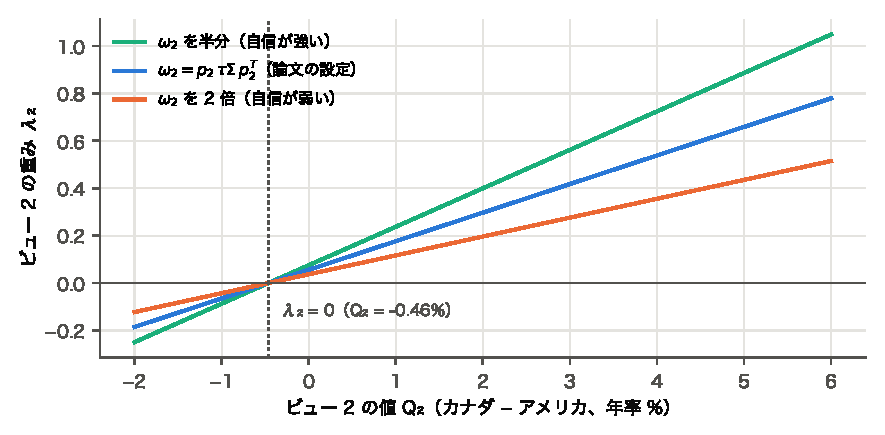
\includegraphics[width=0.94\linewidth]{fig_lambda.pdf}
\caption{ビュー 2 の重み $\lambda_2$ と、ビュー 2 の値 $Q_2$、不確かさ $\omega_2$ の関係（ビュー 1 は 5\% で固定）。}
\label{fig:lambda}
\end{figure}

\section{この章のまとめ}

\begin{keybox}
\begin{itemize}
\item BL の最適比率は $w^* = (\weq + P\T\Lambda)/(1 + \tau)$ で、「市場の比率」＋「ビューのポートフォリオ」である。ビューに出てこない資産は動かない。
\item 重みは $\Lambda = (\delta A)^{-1}(Q - P\Pi/(1 + \tau))$。ビューの驚きに比例し、不確かさ（$\Omega/\tau$）とビューのポートフォリオのリスク（$P\Sigma P\T$）で割られる。
\item 驚き $Q - P\Pi$ が同じでも、自信が弱い、またはリスクの大きいポートフォリオについてのビューは、小さな重みしか持たない。
\item この形は、制約のない最適化のときだけ成り立つ。空売りの禁止などの制約を付けると、比率は数値計算でしか求まらない（\chapref{ch:practice}）。
\end{itemize}
\end{keybox}

% ============================================================
\chapter{実際に使うときの論点}\label{ch:practice}

He と Litterman の結果は、制約のない最適化と、年率のきれいな入力を前提にしている。本プロジェクトのような実際の計算では、いくつかの点で前提が変わる。この章では、その論点を G7 の例で確かめる。

\section{制約を付ける}

実際の運用では、比率の合計を 1 にし、空売りを禁止することが多い。最適化は
\begin{equation}
\max_w\ w\T\mub - \frac{\delta}{2}w\T\Sp w
\qquad \text{条件：}\ \one\T w = 1,\ w \ge 0
\label{eq:qp}
\end{equation}
になる。目的関数が 2 次式で、条件が 1 次式なので、二次計画問題と呼ばれる。式~\eqref{eq:hl} のような公式はなく、数値計算で解く。

\begin{table}[htbp]
\centering
\caption{例 2 のビューで、最適化の条件を変えたときの比率（\%）。}
\label{tab:constraints}
\small\tabin{constraints}
\end{table}

\tabref{tab:constraints} の列は、左から、市場の比率、制約なし（$\Sigma + M$ を使う、He と Litterman の形）、制約なし（$\Sigma$ を使う）、合計 1 のみ、合計 1 と空売りなし、である。空売りを禁止すると、フランスとイギリスは 0 になる。ドイツを買う資金を、フランスとイギリスの売りでまかなえなくなるので、ドイツの比率も \V{lo.GER}\% に下がる。カナダ（\V{lo.CAN}\%）とアメリカ（\V{lo.USA}\%）は、制約なしとほぼ同じである。

制約を付けると、「ビューに出てこない資産は動かない」という性質は厳密には成り立たない。日本やオーストラリアの比率も、条件を満たすために少し動く。それでも、ビューの向きと強さが比率に表れるという大筋は変わらない。

\section{$\Sigma + M$ か $\Sigma$ か}

He と Litterman は、最適化に予測の共分散 $\Sp = \Sigma + M$ を使う。一方、多くの実装（本プロジェクトを含む）は、最適化に $\Sigma$ をそのまま使う。$\Sigma$ を使うと、制約のない比率は
\begin{equation}
w = (\delta\Sigma)^{-1}\mub
= \weq + \frac{\tau}{\delta}P\T\left(P\tau\Sigma P\T + \Omega\right)^{-1}\left(Q - P\Pi\right)
\label{eq:wsigma}
\end{equation}
となる（式~\eqref{eq:blupdate} に $(\delta\Sigma)^{-1}$ を掛けて、$(\delta\Sigma)^{-1}\Pi = \weq$ を使う）。こちらも「市場の比率＋ビューのポートフォリオ」の形で、市場の部分が $1/(1+\tau)$ 倍されない。重みが 0 になる境目は、ちょうど $Q = P\Pi$ である。

\tabref{tab:constraints} のとおり、2 つの違いは主に全体の大きさ（$1/(1 + \tau)$）で、中身の配分はほとんど変わらない。合計 1・空売りなしの条件では、$\Sigma$ を使った場合との差は最大でも \V{lo.diffSSp}\% だった。$\tau$ が小さければ $M$ は $\Sigma$ に比べて小さいので、どちらを使っても結果は近い。

\section{$\tau$ の役割}\label{sec:tau}

\secref{sec:update} の最後で見たように、事後の期待リターン $\mub$ は、$\tau\Sigma$ と $\Omega$ の比だけで決まる。そのため、$\tau$ の効き方は $\Omega$ の決め方によって大きく変わる。

\paragraph{$\Omega$ を $\tau$ に比例させる場合（He と Litterman）}
式~\eqref{eq:omegahl} では $\Omega = \tau\,\diag(P\Sigma P\T)$ なので、$\tau$ は $\mub$ の式から消える。\tabref{tab:tau} のとおり、$\tau$ を 0.01 から 1 まで変えても $\mub$ はまったく変わらず、$\tau$ は $\Sp$ を通じて比率の全体の大きさ（合計 $1/(1 + \tau)$）だけを変える。

\begin{table}[htbp]
\centering
\caption{例 2 で $\tau$ を変えたとき（$\Omega = \diag(P\tau\Sigma P\T)$、年率 \%）。}
\label{tab:tau}
\small\tabin{tau}
\end{table}

\paragraph{$\Omega$ を固定する場合（本プロジェクト）}
$\Omega$ を $\tau$ と無関係に決めると、$\tau$ はビューの採用率を直接決める。\tabref{tab:taufixed} は、例 2 の $\Omega$（$\tau = 0.05$ で決めたもの）を固定して $\tau$ だけを変えた結果である。ビュー 1 の採用率は 0.17 から 0.83 まで動く。

\begin{table}[htbp]
\centering
\caption{例 2 の $\Omega$ を固定して $\tau$ だけを変えたとき（年率 \%）。}
\label{tab:taufixed}
\small\tabin{tau_fixedomega}
\end{table}

本プロジェクトでは、$\Omega$ は LLM の回答の分散で、$\tau$ とは関係なく決まる。そのため $\tau = 0.025$ という値は、「LLM の予想をどれだけ信じるか」を直接決める係数になっている。元論文の第 2 版が、検証用の期間で $\tau$ を選び直しているのは、このためだと考えられる。

\section{単位をそろえる}

BL の式は、どの単位で書いても成り立つ。ただし、すべての量を同じ単位にそろえる必要がある。

\begin{center}
\small
\begin{tabular}{p{2.4cm}p{4.8cm}p{5.6cm}}
\toprule
量 & He と Litterman の例 & 本プロジェクト \\
\midrule
$\Sigma$ & 年率のリターンの共分散 & 日次リターンの共分散 \\
$\Pi$ & 年率の超過リターン & 1 日あたりの超過リターン \\
$Q$ & 年率の超過リターン & LLM が答えた平均日次リターン $-$ 1 日あたりの無リスク金利 \\
$\Omega$ & 年率のリターンの 2 乗の単位 & 日次リターンの回答の分散 \\
$\delta$ & 単位なし（2.5） & 単位なし（2.5）。日次でも年率でも同じ値（第 2 章） \\
$\tau$ & 単位なし（0.05） & 単位なし（0.025） \\
\bottomrule
\end{tabular}
\end{center}

単位がずれると、計算は動いても結果は意味を失う。本プロジェクトの元の実装では、日次のリターンから年率の金利 0.02 をそのまま引いていた（\secref{sec:original}）。

\section{共分散の推定}\label{sec:lw}

BL は $\Sigma$ を 3 か所で使う。均衡リターン（$\Pi = \delta\Sigma\weq$）、事後の期待リターン（$\tau\Sigma$）、最適化である。G7 の例は 7 資産で、長い期間のデータから $\Sigma$ を推定できる。しかし \SP{} の約 500 銘柄では、事情が違う。

$T$ 日分の日次リターンから作った $N \times N$ の標本共分散行列 $S$ の階数は、高々 $T - 1$ である。$T \le N$ なら $S$ は特異で、逆行列がない。1 年分（252 日）でも 500 銘柄には足りない。逆行列がない行列で最適化すると、「分散が 0 に見える組み合わせ」に比率が流れ込む。

Ledoit と Wolf（2004）の縮小推定は、標本共分散を単純な形の行列 $F$ に寄せる。
\begin{equation}
\hat\Sigma = (1 - \alpha)\,S + \alpha\,F,\qquad F = \frac{\mathrm{tr}(S)}{N}\,I
\label{eq:lw}
\end{equation}
$F$ は、全銘柄の分散を平均値にそろえ、共分散を 0 にした行列である。寄せる強さ $\alpha$ は、真の共分散からの誤差（フロベニウスノルムの 2 乗の期待値）が最小になるように、データから決める。$\alpha > 0$ なら $\hat\Sigma$ は必ず正定値になる。本プロジェクトは scikit-learn の \code{LedoitWolf} をこの設定で使っている。判断日 \V{pj.date} の \V{pj.N} 銘柄・\V{pj.days} 日では、$\alpha = \V{all.alpha}$ だった。

% ============================================================
\chapter{本プロジェクトの計算}\label{ch:project}

この章では、本プロジェクトの BL の戦略（\code{blm/strategies.py} の \code{black\_litterman}）が、ここまでの式のどれをどう使っているかを確かめ、実際のデータで 1 段ずつ計算する。

\section{計算の流れ}

\begin{figure}[htbp]
\centering
\begin{adjustbox}{max width=\linewidth}
\begin{tikzpicture}[x=1cm,y=1cm]
\node[box=c3] (px)  at (0,0)     {株価\\（判断日までの 252 取引日）};
\node[box=c3] (sig) at (3.35,0)  {共分散 $\hat\Sigma$\\（Ledoit-Wolf）};
\node[box=c3] (cap) at (0,-1.55) {時価総額\\（判断日）};
\node[box=c3] (w)   at (3.35,-1.55) {市場の比率\\$\weq$};
\node[box=c3] (pi)  at (6.7,-1.55) {均衡リターン\\$\Pi = \delta\hat\Sigma\weq$};
\node[box=c4] (mon) at (0,-3.1)  {判断月の日次リターン\\と会社情報};
\node[box=c4] (llm) at (3.35,-3.1) {LLM に 30 回聞く\\（gpt-4o-mini）};
\node[box=c4] (q)   at (6.7,-3.1)  {$Q$ = 回答の平均 $- r_f$\\$\Omega$ = diag(回答の分散)};
\node[box=c1] (bl)  at (10.05,-2.325) {BL の事後リターン\\$\mub$（$P = I$）};
\node[box=c1] (opt) at (13.4,-2.325) {最適化\\合計 1・空売りなし};
\node[box=c2] (wt)  at (13.4,-4.0) {比率 $w$};
\draw[arr] (px) -- (sig);
\draw[arr] (cap) -- (w);
\draw[arr] (w) -- (pi);
\draw[arr] (sig.south east) -- (pi.north west);
\draw[arr] (mon) -- (llm);
\draw[arr] (llm) -- (q);
\draw[arr] (pi.east) -- (bl.west);
\draw[arr] (q.east) -- (bl.west);
\draw[arr] (bl) -- (opt);
\draw[arr] (opt) -- (wt);
\draw[arr,dashed] (sig.east) -| node[lab,pos=0.25,above]{$\hat\Sigma$ は BL と最適化でも使う} (opt.north);
\draw[arr,dashed] (sig.east) -| (bl.north);
\end{tikzpicture}
\end{adjustbox}
\caption{本プロジェクトの BL の計算。緑は市場のデータ、黄は LLM、青は計算、橙は出力。}
\label{fig:flow}
\end{figure}

時間の決まりは次のとおりである。判断日は $t$ 月の最後の取引日で、使うのはその日までの情報だけである。LLM には $t$ 月の日次リターン（前月末の終値から計算した約 20 日分）と会社情報（ティッカー、社名、GICS のセクターとサブ業種）を渡し、$t+1$ 月の平均日次リターンを答えさせる。比率は判断日の終値で買い、$t+1$ 月の最後の取引日まで持つとして評価する。

\section{He と Litterman の記号とコードの対応}

\begin{center}
\small
\begin{tabular}{p{1.4cm}p{5.8cm}p{5.6cm}}
\toprule
記号 & 本プロジェクトでの中身 & コード \\
\midrule
$\Sigma$ & 判断日までの 252 取引日の日次リターンを Ledoit-Wolf で縮小推定 & \code{shrunk\_covariance(inputs.returns)} \\
$\weq$ & 判断日の時価総額の比率（対象の銘柄の中で合計 1） & \code{inputs.market\_weights} \\
$\delta$ & 2.5（\code{BLM\_RISK\_AVERSION}） & \code{config.RISK\_AVERSION} \\
$\Pi$ & $\delta\hat\Sigma\weq$（1 日あたりの超過リターン） & \code{implied\_returns(...)} \\
$P$ & 単位行列 $I$（全銘柄に絶対的なビュー） & 式の中で省略 \\
$Q$ & 30 回答の平均 $-$ 1 日あたりの無リスク金利 & \code{inputs.view\_mean - inputs.risk\_free\_daily} \\
$\Omega$ & 30 回答の分散（母分散）を並べた対角行列 & \code{np.diag(view\_variance)} \\
$\tau$ & 0.025（\code{BLM\_TAU}） & \code{config.TAU} \\
$\mub$ & 更新形~\eqref{eq:blupdate} で $P = I$ & \code{posterior\_returns(...)} \\
最適化 & 式~\eqref{eq:qp} で、$\Sp$ の代わりに $\hat\Sigma$ & \code{optimize(...)}（CVXPY と Clarabel） \\
\bottomrule
\end{tabular}
\end{center}

無リスク金利 $r_f$ は、判断日の 3 か月物米国債の利回り（\code{\^{}IRX}）を 100 で割り、252 で割って 1 日あたりにしたものである。LLM はリターンそのものを答えるので、$r_f$ を引いて超過リターンにそろえる。

対象の銘柄は、判断日に指数に在籍し、LLM の回答と時価総額があり、252 日のうち半分以上の日に株価がある銘柄である。上場前の日のリターンは、その日のほかの銘柄の平均で埋めている。

\section{$P = I$ のときの式}

全銘柄に絶対的なビューを 1 つずつ置くので、$P = I$（$K = N$）である。更新形~\eqref{eq:blupdate} は
\begin{equation}
\mub = \Pi + \tau\Sigma\left(\tau\Sigma + \Omega\right)^{-1}\left(Q - \Pi\right)
\label{eq:blI}
\end{equation}
になる。これが \code{posterior\_returns} の中身である（リスト~\ref{lst:bl}）。

もし $\Sigma$ が対角行列（銘柄どうしが無相関）なら、式~\eqref{eq:blI} は銘柄ごとに分かれて
\begin{equation}
\mub_i = \Pi_i + k_i\,(Q_i - \Pi_i),\qquad k_i = \frac{\tau\sigma_i^2}{\tau\sigma_i^2 + \omega_i}
\label{eq:ki}
\end{equation}
となり、1 資産の式~\eqref{eq:adoption} と同じになる。実際には相関があるので、銘柄 $i$ の $\mub_i$ には、ほかの銘柄のビューの驚き $Q_j - \Pi_j$ も入ってくる。それでも $k_i$ は「その銘柄のビューがどれくらい採用されるか」のよい目安になる。この資料では $k_i$ を「目安の採用率」と呼ぶ。

He と Litterman の形~\eqref{eq:hl} は、$P = I$ なら $w^* = (\weq + \Lambda)/(1 + \tau)$ で、各銘柄がそれぞれ 1 つのビューのポートフォリオになる。$\Lambda_i$ は、銘柄 $i$ を市場の比率からどれだけ増やすか（減らすか）を表す。本プロジェクトのように最適化で $\Sigma$ を使う場合は、式~\eqref{eq:wsigma} から
\begin{equation}
w = \weq + \frac{\tau}{\delta}\left(\tau\Sigma + \Omega\right)^{-1}(Q - \Pi)
\label{eq:wsigmaI}
\end{equation}
である（制約がない場合）。

\section{5 銘柄で計算する}\label{sec:five}

実際の計算は約 490 銘柄で行うが、それでは途中の数字を追えない。ここでは、判断日 \V{pj.date} に、Apple（AAPL）、NVIDIA（NVDA）、JPMorgan Chase（JPM）、Exxon Mobil（XOM）、Johnson \& Johnson（JNJ）の 5 銘柄だけを対象にして、同じ計算を行う。データとコードは本番と同じで、対象の銘柄だけが違う。LLM は 2025 年 1 月の日次リターン（\V{pj.mdays} 日分）を見て、2 月の平均日次リターンを答えている。

\subsection{手順 1：過去 1 年のリターン}

判断日までの \V{pj.days} 取引日の日次リターンの平均と標準偏差、相関を\tabref{tab:pjstats}と\tabref{tab:pjcorr}に示す。

\begin{table}[htbp]
\centering
\caption{5 銘柄の過去 \V{pj.days} 取引日の日次リターン。年率は平均を 252 倍、標準偏差を $\sqrt{252}$ 倍したもの。}
\label{tab:pjstats}
\small\tabin{pj_stats}
\end{table}

\begin{table}[htbp]
\centering
\caption{5 銘柄の日次リターンの相関。}
\label{tab:pjcorr}
\small\tabin{pj_corr}
\end{table}

過去 1 年の平均をそのまま期待リターンにすると、NVDA の年率 81\% のような値になる。これを平均分散最適化に入れるのが、本プロジェクトの「平均分散（過去 1 年）」の戦略で、\secref{sec:mvweak} の弱点がそのまま出る。

\subsection{手順 2：共分散の縮小推定}

5 銘柄・252 日なら標本共分散でも逆行列はあるが、本番と同じく Ledoit-Wolf を使う。この 5 銘柄では、寄せる強さは $\alpha = \V{pj.alpha5}$、寄せる先の分散（5 銘柄の分散の平均）は $\V{pj.target5} \times 10^{-4}$ だった。\tabref{tab:pjlw} のとおり、分散は平均に向かって少し寄り（NVDA は下がり、ほかは上がる）、共分散は $1 - \alpha$ 倍に縮む。

\begin{table}[htbp]
\centering
\caption{標本共分散と Ledoit-Wolf の推定（日次、$\times 10^{4}$）。}
\label{tab:pjlw}
\small\tabin{pj_lw}
\end{table}

scikit-learn の \code{LedoitWolf} は、標本共分散を $T - 1$ ではなく $T$ で割って作る（最尤推定）。そのため\tabref{tab:pjlw}の「標本」は、pandas の \code{cov()} の値とわずかに違う。

\subsection{手順 3：市場の比率と均衡リターン}

5 銘柄の時価総額の比率を、合計 1 になるように直し、$\Pi = 2.5\,\hat\Sigma\weq$ を計算する（\tabref{tab:pjprior}）。

\begin{table}[htbp]
\centering
\caption{5 銘柄の市場の比率と均衡リターン（1 日あたり）。$\beta_i$ は 5 銘柄の市場に対するベータ。}
\label{tab:pjprior}
\small\tabin{pj_prior}
\end{table}

\begin{exbox}[計算例 7.1：AAPL の均衡リターン]
$(\hat\Sigma\weq)_{\mathrm{AAPL}} = \sum_j \hat\Sigma_{\mathrm{AAPL},j}\,w_j = \V{pj.SwAAPL} \times 10^{-4}$ なので
\[
\Pi_{\mathrm{AAPL}} = 2.5 \times \V{pj.SwAAPL} \times 10^{-4} = \V{pj.PiAAPL}\% \text{（1 日あたり）}.
\]
5 銘柄の市場の分散は $\sigma_m^2 = \V{pj.var5} \times 10^{-4}$ で、$\Pi_m = 2.5\sigma_m^2 = \V{pj.Pim5}\%$／日である。単純に年率に直すと、期待超過リターン \V{pj.Pim5year}\%、標準偏差 \V{pj.sigm5year}\% になる。
\end{exbox}

JNJ の均衡リターンは \V{pj.PiJNJ}\% と負である。この 5 銘柄だけの「市場」は AAPL と NVDA が 8 割を占め、JNJ は NVDA と負の相関（$-0.42$）を持つので、ベータが負（\V{pj.betaJNJ}）になる。市場の値動きを打ち消す側の資産は、それだけでリスクを減らす価値があるので、低い期待リターンでも持たれる、という理屈である。均衡リターンは、対象にする銘柄の集まりによって変わる。

\subsection{手順 4：LLM の回答からビューを作る}

LLM には、同じ質問を 1 回のリクエストで 30 回分答えさせる（temperature 1.0）。AAPL の 30 個の回答を\tabref{tab:pjaapl}に示す。

\begin{table}[htbp]
\centering
\caption{AAPL についての 30 個の回答（翌月の平均日次リターン、\%）。}
\label{tab:pjaapl}
\footnotesize\tabin{pj_aapl}
\end{table}

30 個の平均は \V{pj.aaplmean}\%、標準偏差は \V{pj.aaplsd}\% である。LLM に渡した 1 月の日次リターンの平均は \V{pj.aaplmon}\% で、回答の平均はこれに近い。5 銘柄の集計を\tabref{tab:pjanswers}に示す。

\begin{table}[htbp]
\centering
\caption{5 銘柄の回答の集計（1 日あたり）。「1 月の平均」は LLM に渡した日次リターンの平均。}
\label{tab:pjanswers}
\small\tabin{pj_answers}
\end{table}

AAPL、JPM、JNJ の回答の平均は 1 月の平均に近い。総合報告書の分析でも、予想は入力した月の平均リターンにおおむね沿っていた（全銘柄での相関は 30 か月の平均で 0.89）。ただし NVDA は、1 月の平均が負なのに回答の平均は正で、例外もある。

ビューは
\[
Q_i = (\text{回答の平均})_i - r_f,\qquad \omega_i = (\text{回答の分散})_i
\]
である。この判断日の無リスク金利は 1 日 \V{pj.rf}\%（年率 \V{pj.rfyear}\%）なので、たとえば $Q_{\mathrm{AAPL}} = \V{pj.aaplmean}\% - \V{pj.rf}\% = \V{pj.QAAPL}\%$、$\omega_{\mathrm{AAPL}} = (\V{pj.aaplsd}\%)^2 = \V{pj.aaplvar} \times 10^{-6}$ である。分散は 30 で割る母分散で、データベースのビュー \code{llm\_view\_stats} が計算している。

\subsection{手順 5：2 つの不確かさを比べる}

ビューがどれくらい採用されるかは、$\omega_i$ と $\tau\hat\Sigma_{ii}$ の比で決まる（式~\eqref{eq:ki}）。\tabref{tab:pjratio} のとおり、5 銘柄の目安の採用率は \V{pj.kmin}〜\V{pj.kmax} で、He と Litterman の 0.5 よりずっと大きい。LLM の回答のばらつきは、均衡の不確かさ（$\tau = 0.025$）よりも小さいので、ビューのほうが信頼される。

\begin{table}[htbp]
\centering
\caption{均衡の不確かさとビューの不確かさ（1 日あたりの 2 乗、$\times 10^{6}$）。}
\label{tab:pjratio}
\small\tabin{pj_ratio}
\end{table}

NVDA は値動きが大きい（$\hat\Sigma_{ii}$ が大きい）ので、均衡の不確かさ $\tau\hat\Sigma_{ii}$ も大きく、採用率が最も高い。値動きの大きい銘柄ほど、均衡リターンは当てにならないとみなされ、ビューに寄る。

\subsection{手順 6：事後の期待リターン}

式~\eqref{eq:blI} で計算した結果を\tabref{tab:pjpost}と\figref{fig:pjpost}に示す。「動いた割合」は $(\mub_i - \Pi_i)/(Q_i - \Pi_i)$ である。更新形（本プロジェクトの関数）と情報形（元の実装の関数）の結果の差は、最大で \V{pj.formdiff} だった。

\begin{table}[htbp]
\centering
\caption{5 銘柄の均衡リターン、ビュー、事後の期待リターン（\%／日）。}
\label{tab:pjpost}
\small\tabin{pj_post}
\end{table}

\begin{figure}[htbp]
\centering
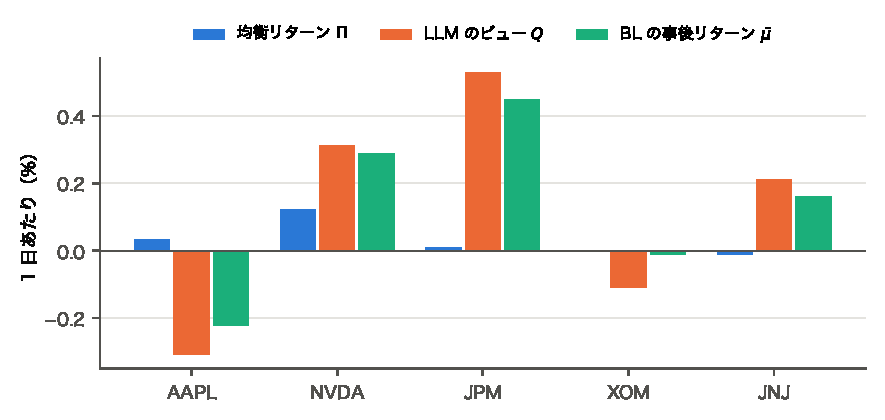
\includegraphics[width=0.94\linewidth]{fig_pj_post.pdf}
\caption{5 銘柄の均衡リターン $\Pi$、LLM のビュー $Q$、事後の期待リターン $\mub$（1 日あたり）。}
\label{fig:pjpost}
\end{figure}

\begin{exbox}[計算例 7.2：AAPL の事後の期待リターン（目安）]
相関を無視した式~\eqref{eq:ki} で計算すると、$\tau\hat\Sigma_{ii} = \V{pj.tsAA} \times 10^{-6}$、$\omega_i = \V{pj.omAA} \times 10^{-6}$ から $k = \V{pj.kAA}$、
\[
\mub_{\mathrm{AAPL}} \approx \V{pj.PiAAPL}\% + \V{pj.kAA} \times (\V{pj.gapAAPL}\%) = \V{pj.diagAAPL}\%
\]
である。行列の式~\eqref{eq:blI} の値は \V{pj.muAAPL}\% で、目安とほぼ同じになる。
\end{exbox}

目安と大きく違うのは XOM である。目安の採用率は \V{pj.kXOM} なのに、実際に動いた割合は \V{pj.moveXOM} しかない。XOM 自身のビューは弱気（$Q = \V{pj.QXOM}\%$）だが、XOM と正の相関を持つ JPM（相関 \V{pj.corrXOMJPM}）と JNJ のビューが強気なので、その情報が相関を通じて XOM の期待リターンを押し上げ、自身の弱気のビューを打ち消している。\secref{sec:update} で見た「驚きが相関を通じて広がる」働きが、ここでも起きている。

\subsection{手順 7：比率}

最後に、$\mub$ を最適化に入れる。結果を\tabref{tab:pjweights}に示す。

\begin{table}[htbp]
\centering
\caption{5 銘柄の比率（\%）。「BL 制約なし」は式~\eqref{eq:wsigmaI}、「合計 1・空売りなし」が本プロジェクトの計算。}
\label{tab:pjweights}
\small\tabin{pj_weights}
\end{table}

まず確かめとして、$\mub$ の代わりに $\Pi$ を入れると、比率は市場の比率に戻る（差は最大 \V{pj.eqcheck}）。

ところが $\mub$ を入れると、本プロジェクトの計算（合計 1・空売りなし）は JPM に \V{pj.wblJPM}\% を入れる。制約のない比率は、合計が \V{pj.wfreesum}\% で、AAPL と XOM を大きく空売りし、JPM と JNJ を何倍も買う。市場の比率を少し調整する、という BL 本来の形にはなっていない。

理由は、期待リターンの差がリスクに比べて大きすぎることである。最適な比率では、持つ銘柄について $\mub_i - \delta(\hat\Sigma w)_i$（リターンからリスクの罰則を引いた、比率を少し増やしたときの得）が等しく、持たない銘柄ではそれ以下になる（ラグランジュの条件。付録 A）。JPM だけを持つ点で計算すると\tabref{tab:pjkkt}になる。

\begin{table}[htbp]
\centering
\caption{JPM に全額を入れた点での、比率を少し増やしたときの得（\%／日）。}
\label{tab:pjkkt}
\small\tabin{pj_kkt}
\end{table}

リスクの罰則 $\delta(\hat\Sigma w)_i$ は、最も大きい JPM でも 1 日 \V{pj.penJPM}\% しかない。一方、$\mub$ の銘柄間の差は 1 日 0.1〜0.7\% ある。罰則が小さすぎて分散する理由がなく、$\mub$ の最も高い銘柄に全額が入る。

He と Litterman の形~\eqref{eq:hl} で見ても、同じことが分かる（\tabref{tab:pjhl}）。G7 の例ではビューの重みは 0.3 前後だったが、ここでは AAPL が \V{pj.lamAAPL}、JPM が \V{pj.lamJPM} で、市場の比率の何倍もの売り買いをビューが求めている。AAPL の驚き $Q - \Pi = \V{pj.gapAAPL}\%$／日は、単純に 252 倍すると年率 $-86\%$、JPM は年率 $+131\%$ に当たる。年率で数 \% の差を言う He と Litterman のビューとは、大きさの桁が違う。

\begin{table}[htbp]
\centering
\caption{He と Litterman の形で見た 5 銘柄の比率（制約なし、$\Sp = \hat\Sigma + M$）。}
\label{tab:pjhl}
\small\tabin{pj_hl}
\end{table}

\section{全銘柄では}

同じ判断日の本番の計算（\V{pj.N} 銘柄）でも、様子は同じである。

\begin{itemize}
\item 縮小推定の強さは $\alpha = \V{all.alpha}$ だった。
\item $\omega_i/(\tau\hat\Sigma_{ii})$ の中央値は \V{all.ratiomed}（四分位 \V{all.ratioq1}〜\V{all.ratioq3}）、目安の採用率の中央値は \V{all.kmed}（四分位 \V{all.kq1}〜\V{all.kq3}）である（\figref{fig:pjadoption}）。実際に動いた割合の中央値は \V{all.movemed} で、目安より大きい。
\item 事後の期待リターンと $Q$ の相関は \V{all.corrQ}、$\Pi$ との相関は \V{all.corrPi} である。$\mub$ はほとんど LLM のビューで決まっている。
\item 均衡リターンの中央値は 1 日 \V{all.Pimed}\%（銘柄間の標準偏差 \V{all.Pisd}\%）、ビューの中央値は 1 日 \V{all.Qmed}\%（同 \V{all.Qsd}\%）で、ビューのばらつきは均衡の 30 倍以上ある。
\item 比率は \V{all.nheld} 銘柄に集中し、実質的な銘柄数（$1/\sum_i w_i^2$）は \V{all.effbl} である。市場の比率は \V{all.effmkt} である。
\end{itemize}

\begin{figure}[htbp]
\centering
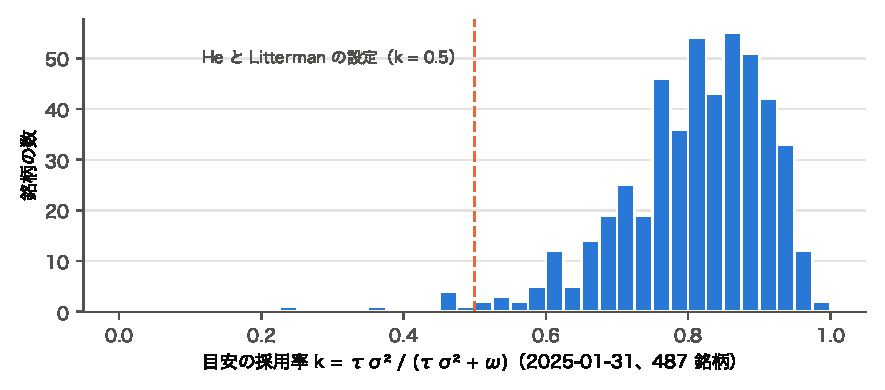
\includegraphics[width=0.94\linewidth]{fig_pj_adoption.pdf}
\caption{全銘柄の目安の採用率 $k_i$ の分布（判断日 \V{pj.date}）。}
\label{fig:pjadoption}
\end{figure}

\begin{table}[htbp]
\centering
\caption{事後の期待リターンが高い 6 銘柄（判断日 \V{pj.date}、全銘柄の計算）。}
\label{tab:alltop}
\small\tabin{all_top}
\end{table}

\tabref{tab:alltop} のとおり、比率を持つのは、事後の期待リターンが最も高い 2 銘柄（VST と CEG）だけである。どちらも、LLM が 1 日 1.6〜1.7\% という予想を出した銘柄である。\V{all.topname} の $Q = \V{all.topQ}\%$／日は、21 日の複利で 1 か月に \V{all.topQmonth}\% の上昇に当たる。この計算は、データベースに保存されている本番の比率と一致する（差は最大 \V{all.storeddiff}\%）。

30 か月の判断日それぞれで、全銘柄の $\omega_i/(\tau\hat\Sigma_{ii})$ の中央値を取ると \V{dates.rmin}〜\V{dates.rmax}、目安の採用率の中央値は \V{dates.kmin}〜\V{dates.kmax} だった（\figref{fig:adoption} の網かけ）。どの月でも、LLM のビューは He と Litterman の設定より強く採用されている。

\section{He と Litterman の設定との違い}

\begin{center}
\small
\begin{tabular}{p{2.8cm}p{4.6cm}p{5.4cm}}
\toprule
項目 & He と Litterman & 本プロジェクト \\
\midrule
ビュー & 少数（1〜3 個）。相対的 & 全銘柄（約 490 個）。絶対的（$P = I$） \\
ビューの大きさ & 均衡との差が年率で数 \% & 均衡との差が 1 日 0.1\%（年率で約 25\%）を超える銘柄が \V{all.shareBig}\% \\
$\Omega$ & $\diag(P\tau\Sigma P\T)$。採用率 0.5 & 回答の分散。採用率の中央値は 0.75〜0.91 \\
$\tau$ & 0.05（$\mub$ には効かない） & 0.025（採用率を直接決める） \\
$\Sigma$ & 与えられた年率の共分散 & 252 日の日次リターンを縮小推定 \\
最適化の共分散 & $\Sigma + M$ & $\hat\Sigma$ \\
制約 & なし & 合計 1・空売りなし \\
単位 & 年率 & 日次 \\
\bottomrule
\end{tabular}
\end{center}

He と Litterman の「市場の比率を、ビューの分だけ動かす」という直観は、ビューの驚き $Q - P\Pi$ が、ビューのポートフォリオのリスクに比べて小さいときに成り立つ。本プロジェクトの計算は、式としては同じ BL だが、ビューが大きく、強く信じられているために、平均分散最適化の弱点（\secref{sec:mvweak}）がそのまま出ている。式~\eqref{eq:lambdasimple} で言えば、$Q - P\Pi$ が大きく、$\Omega/\tau$ が小さいので、$\Lambda$ が非常に大きくなる。

改善の方向は、この式から読み取れる。$Q - \Pi$ を小さくする（予想を当たり具合に合わせて縮める）、$\Omega$ を大きくする（回答のばらつきではなく、予測の外れ方から決める）、$\tau$ を小さくする、比率のずれに上限を付ける、のいずれかである。どれを選ぶかは総合報告書の「次に決めること」で検討しており、この資料では立ち入らない。

\section{元の実装との違い}\label{sec:original}

本プロジェクトには、元論文の公式実装と同じ計算を再現した戦略 \code{black\_litterman\_original} もある。ここまでの式から見ると、違いは次のとおりである。

\begin{center}
\small
\begin{tabular}{p{2.4cm}p{5.2cm}p{5.2cm}}
\toprule
 & 元の実装 & 本プロジェクト \\
\midrule
共分散 & 判断月の約 20 日分の標本共分散 & 252 日分の縮小推定 \\
事前の期待リターン & $\beta_i \times \mathrm{mean}(R_m - 0.02)$。日次のリターンから年率の金利を引く & $\Pi = \delta\hat\Sigma\weq$ \\
ビュー & $Q$ = 回答の平均（金利を引かない） & $Q$ = 回答の平均 $- r_f$ \\
事後の式 & 情報形~\eqref{eq:blinfo}、疑似逆行列 & 更新形~\eqref{eq:blupdate} \\
最適化 & $w\T\Sigma w - 0.1\,w\T\mub$ を SciPy（SLSQP、標準の設定）で最小化 & $w\T\mub - \frac{\delta}{2}w\T\hat\Sigma w$ を二次計画の解法で最大化 \\
\bottomrule
\end{tabular}
\end{center}

元の実装の目的関数は、0.1 で割って符号を変えると $w\T\mub - 10\,w\T\Sigma w$ の最大化と同じで、$\delta/2 = 10$、つまり $\delta = 20$ の平均分散最適化である。同じ 5 銘柄で元の実装の計算を行った結果を\tabref{tab:pjorig}に示す。

\begin{table}[htbp]
\centering
\caption{元の実装の計算（5 銘柄、\%／日）。最後の 2 列は比率（\%）。}
\label{tab:pjorig}
\tabin{pj_orig}
\end{table}

\begin{itemize}
\item \textbf{事前の期待リターン}：1 月の 5 銘柄の市場の平均リターンは 1 日 \V{or.mktmean}\% で、ここから 0.02（年率 2\% のつもりの値）を引くと \V{or.prem}\% になる。AAPL の事前の期待リターンは 1 日 \V{or.PiAAPL}\% で、「毎日 1\% 近く下がる」という出発点である。
\item \textbf{採用率}：共分散が約 20 日分の標本共分散なので、ビューへの寄り方も変わる。XOM を除けば、事後の値は $Q$ の側に大きく寄っている。
\item \textbf{最適化}：SciPy の解法は \V{or.nit} 回の反復で「成功」と報告して止まり、比率は出発点（全銘柄 20\%）のままだった。目的関数の値は \V{or.f0} で、JPM だけを持つ点の \V{or.fexact} のほうがずっと良い。目的関数の値が $10^{-5}$〜$10^{-4}$ 程度と小さいため、標準の止める基準ではすぐに収束したと判定されたと考えられる。同じ目的関数を最後まで解くと、JPM に \V{or.wJPMexact}\% になる。
\end{itemize}

\subsection{$\Omega$ に 0 があるときの違い}\label{sec:pinv}

情報形は $\Omega^{-1}$ を使う。元の実装は、逆行列の代わりに疑似逆行列（\code{numpy.linalg.pinv}）を使うので、$\omega_i = 0$（30 個の回答がすべて同じ）の銘柄があっても計算は止まらない。しかし疑似逆行列では、0 の逆数は 0 として扱われる。これは「精度 0」、つまり\textbf{不確かさが無限大}という意味になり、本来の「完全な自信」と正反対になる。

2 銘柄で確かめる。$\Pi = (0.03\%, 0.03\%)$、$Q = (0.2\%, 0.2\%)$、$\omega = (10^{-6},\ 0)$、日次の分散 $4 \times 10^{-4}$、共分散 $10^{-4}$、$\tau = 0.025$ とする。更新形では、$\omega_B = 0$ の銘柄 B は $\mub_B = \V{z.muB}\%$ で、ビューがそのまま成り立つ。疑似逆行列を使う情報形では $\mub_B = \V{z.muBo}\%$ で、B 自身のビューは無視され、A のビューから相関を通じて少し動いただけになる。

本プロジェクトのデータでは、回答の分散の最小値は \V{z.minvar} で、0 になった銘柄はなかった。ただし temperature を下げると回答がそろいやすくなるので、注意が必要である。

% ============================================================
\chapter{まとめ}\label{ch:summary}

\begin{keybox}[式の流れ]
\begin{enumerate}
\item 平均分散最適化：$w^* = (\delta\Sigma)^{-1}\mu$。$\mu$ に敏感で、$\mu$ の推定は難しい。
\item 均衡リターン：$\Pi = \delta\Sigma\weq$。これを入れると市場の比率に戻る。CAPM の $\beta_i\Pi_m$ と同じ。
\item 事前の見方：$\mu \sim \mathcal{N}(\Pi, \tau\Sigma)$。
\item ビュー：$P\mu = Q + \varepsilon$、$\varepsilon \sim \mathcal{N}(0, \Omega)$。
\item 事後の期待リターン：$\mub = \Pi + \tau\Sigma P\T(P\tau\Sigma P\T + \Omega)^{-1}(Q - P\Pi)$。
\item 最適比率（制約なし）：$w^* = (\delta\Sp)^{-1}\mub = (\weq + P\T\Lambda)/(1 + \tau)$、$\Lambda = (\delta A)^{-1}(Q - P\Pi/(1 + \tau))$。
\end{enumerate}
\end{keybox}

\begin{keybox}[He と Litterman から分かること]
\begin{itemize}
\item BL の比率は「市場の比率」＋「ビューのポートフォリオ」で、ビューに出てこない資産は動かない。
\item ビューの重みは、驚き $Q - P\Pi$ に比例し、自信（$\Omega$ の小ささ）とともに大きくなる。
\item ビューの値ではなく、均衡との差が効く。$\tau$ と $\Omega$ は比だけが効く。
\end{itemize}
\end{keybox}

\begin{keybox}[本プロジェクトの計算について分かること]
\begin{itemize}
\item コードは、He と Litterman の BL の式を $P = I$ で使い、$\Sp$ の代わりに $\hat\Sigma$ で、合計 1・空売りなしの最適化をしている。式としては正しい。
\item ビューの採用率は、回答のばらつき $\omega_i$ と $\tau\hat\Sigma_{ii}$ の比で決まり、中央値で 0.75〜0.91 と、He と Litterman の 0.5 より高い。
\item ビューの大きさ（均衡との差）が、リスクに比べて桁違いに大きい。そのため、最適化は事後の期待リターンが最も高い 1〜2 銘柄に集中する。
\item 元の実装は、単位の誤り、20 日分の共分散、途中で止まる最適化が重なって、結果が分散して見えていた。
\end{itemize}
\end{keybox}

\section*{コードを読むときの確認事項}

\begin{itemize}\small
\item $\Pi$、$Q$、$\Omega$、$\Sigma$ の単位（日次か年率か、超過リターンか）はそろっているか。$Q$ から無リスク金利を引いているか。
\item $\Omega$ は $\tau\Sigma$ の対角成分と比べてどれくらいか（採用率）。
\item $\Pi$ を最適化に入れたとき、市場の比率に戻るか。最適化は最後まで解けているか。
\item 比率は、ビューの向きに沿って市場の比率から動いているか。極端な集中になっていないか。
\end{itemize}

% ============================================================
\appendix
\chapter{行列の公式}\label{app:formulas}

\section{ベクトルでの微分}

$a$ を定数ベクトル、$B$ を定数の対称行列とすると
\[
\frac{\partial}{\partial x}(a\T x) = a,\qquad
\frac{\partial}{\partial x}(x\T B x) = 2Bx .
\]
成分で書くと、$x\T Bx = \sum_i\sum_j B_{ij}x_i x_j$ を $x_k$ で微分して $\sum_j B_{kj}x_j + \sum_i B_{ik}x_i = 2(Bx)_k$ である。式~\eqref{eq:mvfree} の導出に使った。

\section{平方完成}

$H$ を対称な正定値行列とすると
\[
x\T Hx - 2x\T h = (x - H^{-1}h)\T H(x - H^{-1}h) - h\T H^{-1}h .
\]
右辺を展開すれば確かめられる。$\exp(-\frac{1}{2}(x\T Hx - 2x\T h))$ に比例する密度は、平均 $H^{-1}h$、共分散 $H^{-1}$ の正規分布である。BL の情報形~\eqref{eq:blinfo} の導出に使った。

\section{Woodbury の公式}

$A$（$N \times N$）と $\Omega$（$K \times K$）が正則で、$G = PAP\T + \Omega$ も正則なら
\[
(A^{-1} + P\T\Omega^{-1}P)^{-1} = A - AP\T G^{-1}PA .
\]
\paragraph{確かめ}
左辺の逆行列に右辺を掛けると
\begin{align*}
(A^{-1} + P\T\Omega^{-1}P)(A - AP\T G^{-1}PA)
&= I - P\T G^{-1}PA + P\T\Omega^{-1}PA \\
&\qquad - P\T\Omega^{-1}(PAP\T)G^{-1}PA \\
&= I + P\T\left[-G^{-1} + \Omega^{-1} - \Omega^{-1}(G - \Omega)G^{-1}\right]PA \\
&= I + P\T\left[-G^{-1} + \Omega^{-1} - \Omega^{-1} + G^{-1}\right]PA = I .
\end{align*}
左辺は $N \times N$ の逆行列だが、右辺は $K \times K$ の逆行列 $G^{-1}$ しか使わない。ビューの数 $K$ が資産の数 $N$ より少ないときに計算が楽になる。式~\eqref{eq:blupdate} の導出に使った。

\section{正規分布の条件付き分布}

$(x, y)$ が同時に正規分布に従い
\[
\begin{pmatrix} x \\ y \end{pmatrix} \sim \mathcal{N}\left(\begin{pmatrix} m_x \\ m_y \end{pmatrix},\ \begin{pmatrix} S_{xx} & S_{xy} \\ S_{yx} & S_{yy} \end{pmatrix}\right)
\]
なら、$y$ を知った後の $x$ の分布は
\[
x \mid y \sim \mathcal{N}\left(m_x + S_{xy}S_{yy}^{-1}(y - m_y),\ \ S_{xx} - S_{xy}S_{yy}^{-1}S_{yx}\right)
\]
である。

\paragraph{BL の公式の別の導き方}
$x = \mu$、$y = Q = P\mu + \varepsilon$ とおく。$\mu \sim \mathcal{N}(\Pi, \tau\Sigma)$ と $\varepsilon \sim \mathcal{N}(0, \Omega)$ が独立なら
\[
m_x = \Pi,\quad m_y = P\Pi,\quad S_{xx} = \tau\Sigma,\quad S_{xy} = \mathrm{Cov}(\mu, P\mu + \varepsilon) = \tau\Sigma P\T,\quad S_{yy} = P\tau\Sigma P\T + \Omega
\]
で、上の公式に入れると、更新形~\eqref{eq:blupdate} と \eqref{eq:blMupdate} がそのまま出てくる。「ビューの値 $Q$ が、均衡から予想される値 $P\Pi$ からずれた分を、$\mu$ と $Q$ の共分散に応じて $\mu$ に反映する」という読み方ができる。カルマンフィルタの更新と同じ形である。

\section{制約付きの最適化の条件}

合計 1・空売りなしの最適化~\eqref{eq:qp} で、目的関数の勾配を $g = \mub - \delta\Sigma w$ とする。$w$ が最適であるための条件（KKT 条件）は、ある数 $\gamma$ について
\[
g_i = \gamma \quad (w_i > 0),\qquad g_i \le \gamma \quad (w_i = 0)
\]
が成り立つことである。比率を持つ銘柄では、比率を少し増やしたときの得 $g_i$ がそろっていて、持たない銘柄では、それより小さい。もし $g_j > \gamma$ の銘柄があれば、ほかの銘柄から少し移すと目的関数が増えるので、最適ではない。\tabref{tab:pjkkt} はこの条件を確かめたものである。

% ============================================================
\begingroup\let\clearpage\relax
\vspace{2\Cvs}
\chapter{本プロジェクトのコード}\label{app:code}
\endgroup

この資料で扱った計算の、本プロジェクトのコードを載せる（2026 年 10 月時点）。

\begin{lstlisting}[language=Python,caption={均衡リターン（\code{blm/equilibrium.py} の一部）}]
def implied_returns(covariance, market_weights, risk_aversion):
    """Excess returns that make the market-cap weights optimal: pi = delta x Sigma x w_market."""
    return risk_aversion * covariance @ market_weights
\end{lstlisting}

\begin{lstlisting}[language=Python,caption={BL の事後の期待リターン（\code{blm/black\_litterman.py}）},label={lst:bl}]
def posterior_returns(prior, covariance, view_mean, view_variance, tau):
    """prior + tau Sigma (tau Sigma + Omega)^-1 (Q - prior), with Omega = diag(view_variance)."""
    tau_sigma = tau * covariance.values
    omega = np.diag(view_variance.values)
    adjustment = tau_sigma @ np.linalg.solve(tau_sigma + omega, (view_mean - prior).values)
    return prior + pd.Series(adjustment, index=prior.index)


def posterior_returns_original(prior, covariance, view_mean, view_variance, tau):
    """The same posterior written as in the original implementation (pseudo-inverses)."""
    inv_tau_sigma = np.linalg.pinv(tau * covariance.values)
    inv_omega = np.linalg.pinv(np.diag(view_variance.values))
    m = np.linalg.pinv(inv_tau_sigma + inv_omega)
    return pd.Series(m @ (inv_tau_sigma @ prior.values + inv_omega @ view_mean.values), index=prior.index)
\end{lstlisting}

\code{posterior\_returns} は式~\eqref{eq:blI}（更新形で $P = I$）、\code{posterior\_returns\_original} は式~\eqref{eq:blinfo}（情報形で $P = I$）である。\code{np.linalg.solve(A, b)} は $A^{-1}b$ を、逆行列を作らずに計算する。

\begin{lstlisting}[language=Python,caption={最適化（\code{blm/optimizer.py} の一部）}]
OBJECTIVE_SCALE = 1e4

def optimize(expected_returns, covariance, risk_aversion):
    """Maximize  w.mu - risk_aversion / 2 x w.Sigma.w   subject to  sum(w) = 1, w >= 0."""
    w = cp.Variable(len(expected_returns))
    objective = expected_returns.values @ w - risk_aversion / 2 * cp.quad_form(w, cp.psd_wrap(covariance.values))
    problem = cp.Problem(cp.Maximize(OBJECTIVE_SCALE * objective), [cp.sum(w) == 1, w >= 0])
    problem.solve(solver=cp.CLARABEL)
    if problem.status != cp.OPTIMAL:
        raise RuntimeError(f"optimization failed: {problem.status}")
    weights = np.clip(w.value, 0, None)
    return pd.Series(weights / weights.sum(), index=expected_returns.index)
\end{lstlisting}

日次のリターンは $10^{-3}$、分散は $10^{-4}$ 程度と小さいので、目的関数を $10^4$ 倍して、解法の許容誤差に比べて十分大きくしている。元の実装の最適化が途中で止まった問題（\secref{sec:original}）への対処でもある。

\begin{lstlisting}[language=Python,caption={BL の戦略（\code{blm/strategies.py} の一部）}]
def black_litterman(inputs):
    """Market equilibrium corrected by the LLM views."""
    covariance = shrunk_covariance(inputs.returns)
    prior = implied_returns(covariance, inputs.market_weights, config.RISK_AVERSION)
    views = inputs.view_mean - inputs.risk_free_daily      # the LLM predicts returns, the prior is in excess returns
    expected = posterior_returns(prior, covariance, views, inputs.view_variance, config.TAU)
    return optimize(expected, covariance, config.RISK_AVERSION)
\end{lstlisting}

\begin{lstlisting}[language=SQL,caption={回答の平均と分散（\code{marketdb/db/schema.sql} のビュー \code{llm\_view\_stats}）}]
CREATE VIEW IF NOT EXISTS llm_view_stats AS
SELECT run_id, as_of_date, symbol,
       COUNT(expected_return) AS n_answers,
       AVG(expected_return)   AS mean_return,
       AVG(expected_return * expected_return) - AVG(expected_return) * AVG(expected_return) AS variance
FROM llm_views
GROUP BY run_id, as_of_date, symbol;
\end{lstlisting}

\section*{この資料の作り直し方}

数値、表、図は \code{BLM解説\_計算.py} がデータベースから計算し、\code{BLM解説\_生成/} に書き出す。リポジトリの直下で次を実行する。

\begin{lstlisting}[language=bash]
.venv/bin/python 資料集/勉強用/BLM解説_計算.py
cd 資料集/勉強用 && tectonic BLM解説.tex
\end{lstlisting}

判断日（\code{DATE}）や 5 銘柄（\code{T5}）を変えれば、別の月・別の銘柄で同じ計算を見られる。本文の文章は数字に合わせて書いているので、変えた場合は文章との食い違いに注意する。

% ============================================================
\section*{参考文献}
\addcontentsline{toc}{section}{参考文献}

\begin{itemize}[leftmargin=1.2em,itemsep=0.4em]
\item Black, F. and R. Litterman (1992). Global Portfolio Optimization. \textit{Financial Analysts Journal}, 48(5), 28--43.
\item He, G. and R. Litterman (1999). The Intuition Behind Black-Litterman Model Portfolios. \textit{Investment Management Research}, Goldman Sachs \& Co. (SSRN 334304)
\item Idzorek, T. (2005). A Step-by-Step Guide to the Black-Litterman Model: Incorporating User-Specified Confidence Levels. Working paper.
\item Ledoit, O. and M. Wolf (2004). A Well-Conditioned Estimator for Large-Dimensional Covariance Matrices. \textit{Journal of Multivariate Analysis}, 88(2), 365--411.
\item Lee, Y. et al. (2025). Integrating LLM-Generated Views into Mean-Variance Optimization Using the Black-Litterman Model. arXiv:2504.14345.（本プロジェクトの元論文）
\item Markowitz, H. (1952). Portfolio Selection. \textit{Journal of Finance}, 7(1), 77--91.
\item Michaud, R. (1989). The Markowitz Optimization Enigma: Is `Optimized' Optimal? \textit{Financial Analysts Journal}, 45(1), 31--42.
\item Satchell, S. and A. Scowcroft (2000). A Demystification of the Black-Litterman Model: Managing Quantitative and Traditional Portfolio Construction. \textit{Journal of Asset Management}, 1(2), 138--150.
\item Theil, H. and A. S. Goldberger (1961). On Pure and Mixed Statistical Estimation in Economics. \textit{International Economic Review}, 2(1), 65--78.
\item Walters, J. (2014). The Black-Litterman Model in Detail. SSRN 1314585.
\item 本プロジェクト：\code{資料集/報告書/LLM-BLM\_総合報告書.pdf}
\end{itemize}

\end{document}
